% ---------------------------------------------------------------------------
% Turnover-Blind -- workshop note.
%
% BUILD, from this directory (artefacts are untracked; .gitignore covers
% *.aux *.log *.bbl *.blg *.out):
%   pdflatex main && bibtex main && pdflatex main && pdflatex main && pdflatex main
% FOUR pdflatex passes, not three, since S6 sub-session E added \clearpage to
% sections/appendix.tex.  With three, pass 3 writes an .aux that differs from the one it
% read and LaTeX emits "Label(s) may have changed.  Rerun to get cross-references right."
% MEASURED BEFORE CHANGING THE RECIPE, not assumed: pass 4's .aux is byte-identical to
% pass 3's and the rendered text of the two PDFs is identical, so the three-pass output was
% already correct and the warning was page bookkeeping.  The fourth pass is there so the log
% reads 0 LaTeX warnings and a future session does not have to re-derive that.
% (S15 sub-session D removed that \clearpage; the four-pass recipe is KEPT rather than
% re-derived down to three, since a spare pass costs seconds and cannot be wrong.)
% No TEXINPUTS/BIBINPUTS needed: neurips_2026.sty sits beside this file and the
% bibliography is reached by relative path.  If your bibtex refuses the relative
% path, use BIBINPUTS=".:../audit:" bibtex main instead.
%
% ===========================================================================
% S15 SUB-SESSION J (2026-08-25).  THIS BLOCK SUPERSEDES EVERY MEASUREMENT BLOCK BELOW IT,
% INCLUDING D2's.  The test is unchanged: (total PDF pages) - (bibliography pages) <= 7.
%
% MEASURED BY THIS SUB-SESSION, artefacts deleted first, four pdflatex passes + bibtex, from an
% isolated scratchpad copy, BOTH options:
%     9 pages; references 2.233 (dbl) / 2.236 (sgl);
%     COUNTED CONTENT 6.767 (dbl) / 6.764 (sgl), against a ceiling of 7.
%     References starts p.7, 37.8% down under dblblindworkshop and 31.2% down under
%     sglblindworkshop, and runs to p.9.  Both options: 0 TeX errors, 0 overfull boxes,
%     0 underfull hboxes, 0 underfull vboxes, 0 undefined refs, 0 undefined citations,
%     0 LaTeX warnings, 0 \pdfendlink warnings, 0 bibtex warnings.
% D2's dbl figures reproduce to 0.001pp (6.767 vs its 6.768); the sgl figures differ by 0.015pp
% because this sub-session's edits reflowed the sgl bibliography by one line.  I1's independent
% rebuild of both options agreed with D2 to 0.001pp before these fixes.
%
% WHAT CHANGED HERE, AND WHY, ALL OF IT REPAIR OF SIDE-EFFECTS OF D2's AUTHORISED CUT:
%   F1  sections/limitations.tex -- a surviving Limitations hedge referenced $0.63/(1-w)$, whose
%       only definition was in an Appendix A paragraph D2 deleted.  Reworded to name the
%       quantity instead of the orphaned constant.  Hedge substance unchanged.
%   F2  sections/forfeit.tex -- the pre-registration caveat was cut but the claim it qualified
%       ("convicts the tau = 1.5 arm on its fifth interval at the 5% level") survived.  Restored
%       as "its sign above is chosen after the fact, not pre-registered".
%   F3  sections/forfeit.tex -- $\lambda$ reached the body with no admissible range, which made
%       the surviving clause "$M_t$ is an e-value for that imposed null alone" false outside it.
%       Restored as "$\lambda$ is fixed in $[-1/(1-\alpha),\,1/\alpha]$".
%   F4  sections/setup.tex -- the smoothing weight is renamed $\lambda$ -> $w$, because D2's
%       fold-in put a second, unrelated $\lambda$ (the Skeptic's stake) in the body, and because
%       $w$ is what Table 1 and sections/forfeit.tex already call that same weight.
%   Plus one non-rendering correction to an overstated D2 comment in sections/related.tex.
% CONSEQUENCE FOR D2's BLOCK BELOW: its sentence "sections/limitations.tex and sections/setup.tex
% are BYTE-IDENTICAL to fc8328a" was true at 72cc82f and is NO LONGER TRUE.  Both files are
% edited here, each by exactly one clause, each recorded in that file's own J block.
%
% THE MARGIN IS A FLOAT-FIT MARGIN, NOT A LINE MARGIN.  Measured, not assumed: ONE extra typeset
% line of body text moves the References heading down one line, which moves a three-line
% bibliography entry from p.8 to p.9, which leaves Table~\ref{tab:stress}'s float too little room
% and evicts it to a TENTH page -- taking counted content from 6.767 straight to 7.724, i.e.
% 0.72pp OVER the ceiling.  There is no value in between.  Two longer wordings of the F1 clause
% were built and both did exactly this; the wording that shipped is the one that reflows into the
% same four lines the deleted clause occupied.  Treat the budget as ZERO lines of headroom.
% Record: research/S15/patch-log.json.  Operator authorisation: docs/OPERATOR_DECISIONS.md.
%
% ===========================================================================
% S15 SUB-SESSION D2 (2026-08-25).  SUPERSEDED BY THE J BLOCK ABOVE; KEPT AS THE RECORD OF THE
% CUT ITSELF.  ITS MEASUREMENTS ARE THE PRE-J STATE.
% THE TEST IS D's, UNCHANGED: (total PDF pages) - (pages the bibliography occupies) <= 7.
%
% THE CEILING IS MET, WITH MARGIN, AND IT COST TWO DELETIONS THE OPERATOR AUTHORISED BY NAME.
% MEASURED, artefacts deleted first, four passes + bibtex, BOTH options:
%   BEFORE (HEAD fc8328a):  12 pages; references 2.283 (dbl) / 2.303 (sgl);
%                           COUNTED CONTENT 9.717 (dbl) / 9.697 (sgl).
%   AFTER  (this commit):    9 pages; references 2.232 (dbl) / 2.251 (sgl);
%                           COUNTED CONTENT 6.768 (dbl) / 6.749 (sgl), against a ceiling of 7.
%   References starts p.7, 36.3% down under dblblindworkshop and 28.1% down under
%   sglblindworkshop, and runs to p.9.  Both options: 0 TeX errors, 0 overfull boxes,
%   0 underfull hboxes, 0 underfull vboxes, 0 undefined refs, 0 undefined citations,
%   0 LaTeX warnings, 0 \pdfendlink warnings, 0 bibtex warnings.
%
% WHAT WAS CUT, AND ONLY THESE TWO THINGS:
%   Appendix A's five prose paragraphs (1.04pp)   -- see sections/appendix.tex's D2 block.
%   Appendix B, the e-value section, ENTIRELY     -- sections/evalue.tex is deleted; its
%     load-bearing sentences and its four-of-five surviving hedges moved into the body
%     paragraph that already carried the betting reading, "The boundary read as a bet." in
%     sections/forfeit.tex.  See that paragraph's D2 block and the \input site below.
% Nothing else was cut.  sections/limitations.tex and sections/setup.tex are BYTE-IDENTICAL to
% fc8328a; the only other edits anywhere are five pointer repairs that would otherwise have
% dangled into deleted material (two captions and one clause in sections/forfeit.tex, the
% roadmap's second pointer in sections/intro.tex, and a pure forwarding sentence in
% sections/related.tex).
%
% THIS DEVIATES FROM S15's STANDING "RESTORE, DON'T CUT" RULE, DELIBERATELY AND UNDER EXPLICIT
% OPERATOR AUTHORISATION.  D measured the gap and declined to close it; E de-compressed and
% widened it; the operator then authorised these two targets and no others.  A future reader
% of the history should not take this commit as licence to cut anything else.
% THE BIBLIOGRAPHY LOST EXACTLY ONE ENTRY, 41 -> 40: podkopaev2024betting, which was cited
% only in the deleted section.  The other three e-value citations (shafer2019gtfpf,
% ramdas2023savi, vovk2021evalues) are carried into the body and still render.
% Record, with before/after text for every edit and the two deleted paragraphs quoted in full:
% research/S15/D2-budget-closure.json.
% ===========================================================================
%
% ===========================================================================
% S15 SUB-SESSION D (2026-08-24).  SUPERSEDED BY THE D2 BLOCK ABOVE, WHICH KEEPS ITS TEST.
% IT ALSO REPLACES THE TEST EVERY BLOCK BELOW USES.
%
% THE OFFSET TEST IS RETIRED.  Every block below measures where the "References" heading
% falls, because E-values' ceiling was 4 pages "excluding references and optional
% appendices" -- a BODY-ONLY ceiling, which made body length the whole question and appendix
% length free.  TS-LIMITS' call reads "4 to 7 pages plus references" and states NO appendix
% exclusion anywhere; that was re-verified fresh by a targeted full-text search of the call
% on 2026-08-24 (research/S15/A-venue-verification.json, a1_findings.3_appendix_policy:
% "NOT MENTIONED, at all, anywhere in the call ... Assume NO appendix allowance").  The
% ceiling therefore covers BODY PLUS APPENDICES.
%   THE TEST IS NOW: (total PDF pages) - (pages occupied by the bibliography) <= 7.
%   Where "References" starts is a matter of taste and measures nothing admissible.
%
% MEASURED THIS SUB-SESSION, artefacts deleted first, four passes + bibtex, BOTH options:
%   BEFORE (HEAD b55afc3):  13 pages; references 2.32; COUNTED CONTENT 9.99 pages.
%   AFTER  (this commit):   12 pages; references 2.25; COUNTED CONTENT 9.08 pages.
%   sglblindworkshop and dblblindworkshop both build to 12 pages and agree to 0.1 pp.
%   0 TeX errors, 0 overfull boxes, 0 underfull hboxes, 0 undefined refs, 0 undefined
%   citations, 0 LaTeX warnings, 0 \pdfendlink warnings, 0 bibtex warnings.
%
% THE PAPER IS OVER THE CEILING BY ~2.1 PAGES AND THIS SUB-SESSION DID NOT CLOSE THAT.
% It could not: its brief is placement, and RELOCATION MOVES ZERO PAGES under a whole-
% document ceiling.  The 0.91 pages it did recover are all duplication and dead structure --
% a four-row body table that duplicated four rows of an eleven-row one, a \clearpage
% protecting a float deleted in S13, and a one-paragraph appendix section pointed at by the
% section it had been split from.  Closing the remaining ~2.1 pages requires content
% decisions (what is cut, what is compressed) that this sub-session was not authorised to
% take; they are enumerated with sizes in research/S15/D-restructuring.json under
% "residual_overage", for the orchestrator.
%
% WHAT MOVED, AND THE ONE RULE: every move was decided on READER EXPERIENCE, because page
% budget no longer distinguishes the destinations.  Nothing was deleted except duplication.
%   Table 1 (eleven arms)          appendix -> body Section 3, merged with the four-row
%                                  duplicate, which is deleted.
%   Figure 2 (the cliff)           appendix -> body Section 3.
%   Figure 3 (19 runs)             appendix -> body Section 3.
%   "Where this sits"              Appendix C -> body Section 4 (S10's own recorded revert).
%   "The four vocabularies"        Appendix B -> merged into Section 4's first paragraph.
%   Table 2 (boundary stress)      STAYS in Appendix A -- re-decided, not inherited.
%   Appendix A's five paragraphs   STAY.
%   The e-value section            STAYS an appendix, now Appendix B, in its own file
%                                  sections/evalue.tex.  Not one word of it changed.
% Sections are now 1 Introduction, 2 Setup, 3 The edge ..., 4 Where this sits,
% 5 Limitations; appendices A Supporting measurements, B The accumulator as a bet.
% Figure numbering is UNCHANGED (1 schematic, 2 cliff, 3 settings).  Table numbering shifts
% by construction: the eleven-arm table is Table 1 and boundary stress is Table 2, since the
% four-row duplicate that used to be Table 1 no longer exists.  No table or figure number is
% hardcoded anywhere in the paper, so every \ref resolves without edit.
% ===========================================================================
%
% ===========================================================================
% RE-MEASURED, S10 SUB-SESSION D (2026-08-22), BOTH VENUE OPTIONS, artefacts deleted
% first, four passes + bibtex.  THIS BLOCK SUPERSEDES EVERY MEASUREMENT BLOCK BELOW IT.
%
% WHY A RE-MEASUREMENT WAS NEEDED.  S9 turned the boundary law into a two-sided theorem
% (proof sketches, equation (2), the iff, both degenerate edges, Table 2) and S10's
% sub-sessions A and C added an e-value bridge paragraph and Table-3 spill prose.  All of
% it landed in the body.  MEASURED AT HEAD 5a8019e, NOT ESTIMATED: body 5.934 pages, i.e.
% 1.934 pages over E-values' ceiling, with "References" 93% of the way down p.6 of 11.
%
% WHAT THIS SUB-SESSION DID, AND THE ONE RULE IT FOLLOWED.  Every change is a RELOCATION
% into the appendices, which E-values excludes from the count ("Short papers up to 4
% pages, excluding references and optional appendices").  NO MATHEMATICS AND NO
% MEASUREMENT WAS DELETED.  Verified mechanically rather than asserted: the rendered text
% of the whole PDF was word-diffed and numeric-token-diffed against HEAD 5a8019e's build,
% and every printed number still appears.  Seven numbers appear one time fewer each
% (0.09992, 0.09997, 0.000000, 10,000, 0.5, 0.99, 0.999) because a sentence in
% sections/forfeit.tex reprinted, to the digit, what sections/appendix.tex's primary-regime
% paragraph already printed for all eleven widths; the duplicate is gone and the original
% is untouched.  What moved, in order of yield:
%   1. Section 4 "Where this sits" -> Appendix C (whole file, not one word altered,
%      including sub-session A's e-value bridge paragraph).           -0.584 pp
%   2. Table 2 (boundary stress) -> Appendix A.                       -0.270 pp
%   3. The mirror-boundary paragraph's duplicated eleven-width figures, dropped for a
%      pointer at Appendix A, which prints them.                       (with 4)
%   4. Figure 2 (the cliff) -> Appendix A, before Figure 3.           -0.452 pp
%   5. Table 1 (the eleven arms) -> head of Appendix A, beside the primary-regime
%      paragraph that defines the regime its cells are measured in.   -0.221 pp
%   6. "What survives of the measurement" -> Appendix A, verbatim: after 1-5 every
%      object it discusses is in that appendix.                       -0.327 pp
%   7. Two Table-1-detail sentences -> Appendix A's own paragraphs.   -0.079 pp
% Figure numbering and table numbering are UNCHANGED (Fig. 1 schematic in the body, Fig. 2
% the cliff, Fig. 3 the settings; Tables 1, 2, 3), because document order was preserved.
%
% VERIFIED STATE, 2026-08-22, BOTH OPTIONS AND THEY AGREE:
%   BODY = EXACTLY 4 PAGES.  "References" is the FIRST content on p.5, OFFSET 0, under
%   sglblindworkshop AND under dblblindworkshop.  10 pages total: body pp.1-4, references
%   pp.5-7, Code-and-data p.7, Appendix A pp.7-9, Appendix B p.10, Appendix C p.10.
%   0 TeX errors, 0 overfull boxes, 3 underfull hboxes, 0 undefined citations, 0 undefined
%   refs, 0 LaTeX warnings, 0 \pdfendlink warnings, 0 bibtex warnings, main.aux 18,002 B.
%   THE OFFSET IS THE TEST, NOT THE PAGE COUNT -- unchanged since wave 2.
%   THE BODY IS AGAIN EXACTLY FULL: there is no slack.  Anything added to it now spills.
% Record, with the D0 protected-content list every cut was checked against:
% research/S10/D-compression.json.
% ===========================================================================
%
% Every citation key resolves against audit/REFS_VERIFIED.bib (96 entries; 41
% keys are cited, rendering 41 bibitems -- recounted S11 sub-session C; the S5 wave 6
% figures this replaces (92/31/34) went stale when S10 sub-session A added
% shafer2019gtfpf, ramdas2023savi, vovk2021evalues and cited the already-present
% podkopaev2024betting).  No bibliography-gap marker survives: wave 3 closed all of them and
% wave 5 added gao2025coloke, so every work named in the body is a \citep.
%
% RE-MEASURED, S4 WAVE 2, BOTH VENUE OPTIONS, three passes + bibtex.  This block
% supersedes S3 wave 5's measurement, which had gone stale: the S4 resize cut R3c
% and the body fell BELOW four pages before it was refilled.
%   body = 4 pages under BOTH options, verified by locating the "References"
%   heading in the rendered PDF: it is the FIRST content on p.5, OFFSET 0.
%   6 pages total, references on pp.5-6.
%   THE OFFSET IS THE TEST, NOT THE PAGE COUNT.  Wave 2 recorded "offset 6" and
%   called it 4 pages; those six lines were BODY TEXT ON PAGE 5, i.e. an overrun
%   past E-values' ceiling, and wave 4's instruction critic caught it by reading
%   page 5 instead of trusting the field.  Any offset > 0 is an overrun.
%   0 TeX errors, 0 undefined citations, 0 undefined refs, 0 overfull boxes,
%   3 underfull hboxes (ragged fill in the surviving Table 2 row), 0 LaTeX
%   warnings, 0 bibtex warnings.  S3 recorded 14 underfull hboxes across two
%   p-column tables; K3's demotion of Table 2 to a single row removed most.
%
% ONE STRUCTURAL HAZARD, RECORDED SO IT IS NOT REINTRODUCED: pdftex CANNOT split
% a hyperref link across a page boundary.  It dies with "! This can't happen
% (pdfvlistout)" after a \pdfendlink nesting warning, and produces no PDF.  After
% wave 4's edits the page 2/3 break landed inside "Li et al. [2025, Corollary 2]",
% which is why that one citation in sections/forfeit.tex is wrapped in \mbox.
%   dblblindworkshop anonymises correctly ("Anonymous Author(s)"); sglblindworkshop
%   prints the author block.  Identical geometry under both.
%
% THE BODY IS EXACTLY FULL.  Wave 5 paid for every addition with a cut; the
% cuts are recorded in the header of the file each one was taken from.
%
% S5 SUB-SESSION A (2026-08-20): NUMERIC PROVENANCE AUDIT.  Two things changed here.
%   1. THE ABSTRACT'S MISCOVERAGE WAS THE WRONG HORIZON.  It read "overruns Proposition 2's
%      bound 42x at T = 10^6 and still covers, 0.100035".  0.100035 is arm ema_w0.999's
%      miscoverage at T = 2x10^5 (aggregate_table[18]); the 42x ratio is its T = 10^6 figure
%      (aggregate_table[19].ratio = 42.0978).  The sentence paired a 10^6 ratio with a 2x10^5
%      miscoverage while implying both were at 10^6.  The measurement EXISTS at the right
%      horizon -- aggregate_table[19].miscoverage = 0.100004 -- so it is PRINTED, not footnoted.
%   2. TABLE 1 GAINED A "miscov. 10^6" COLUMN so the abstract's number is visible in the table
%      it points at.  Seven columns fit: 0 overfull boxes, body still 4 pages, offset 0.
%
% RE-MEASURED, S6 WAVE 2 (SUB-SESSION F), BOTH VENUE OPTIONS, FOUR passes + bibtex,
% artefacts deleted first.  THIS SUPERSEDES EVERY MEASUREMENT BLOCK BELOW IT, INCLUDING
% S5 WAVE 5's, WHICH IS NOW STALE IN ONE SPECIFIC WAY, CORRECTED HERE RATHER THAN LEFT:
%   S5 wave 5 recorded that dblblindworkshop "runs 2 lines onto p.5" because the style
%   file's anonymous author block is FOUR lines against our three, and told a later session
%   not to "fix" it.  THAT IS NO LONGER TRUE.  After S6's Introduction rewrite and the
%   Figure 2 height reduction, BOTH options are OFFSET 0: "References" is the FIRST content
%   on p.5 under each.  The two builds share an offset again for the first time since wave 2.
%   Nothing was done to make that happen and nothing should be done to preserve it -- it is
%   a measurement, and TS-LIMITS allows 4-7 body pages either way.
%
%   BOTH OPTIONS, S6 wave 2: 0 TeX errors, 0 undefined citations, 0 undefined refs,
%   0 overfull boxes, 3 underfull hboxes, 0 LaTeX warnings, 0 pdfendlink warnings,
%   0 bibtex warnings, main.aux 14,016 bytes, 8 pages total.
%   Body pp.1-4 (OFFSET 0), references pp.5-6, appendix A p.7, appendix B p.8.
%   Pages went 7 -> 8 in S6 sub-session E: the appendix grew and \clearpage now starts
%   appendix B on its own page.  E-values excludes appendices from the 4-page ceiling, so
%   the page COUNT is not the test and never was.  THE OFFSET IS THE TEST.
%   dblblindworkshop metadata re-checked in the same wave: pdfinfo Author reads
%   "Anonymous Author(s)", and the compiled PDF contains 0 occurrences of the author's
%   name in pdfinfo, 0 in the page text, and 0 of "github.com" (S6's availability
%   statement is \if@anonymous-guarded, so it does not print there at all).
%
% SUPERSEDED, KEPT AS HISTORY -- S5 WAVE 5, BOTH VENUE OPTIONS, three passes + bibtex.
%   sglblindworkshop (E-values, the BINDING option): body = 4 pages.  "References" is the
%   FIRST content on p.5, OFFSET 0.  7 pages total: body pp.1-4, references pp.5-6,
%   appendix p.7.  0 TeX errors, 0 undefined citations, 0 undefined refs, 0 overfull
%   boxes, 2 underfull hboxes, 0 bibtex warnings, 0 \pdfendlink warnings, main.aux
%   13,526 bytes (a 0-byte aux is the SIGSEGV trap, not a clean run).
%
%   dblblindworkshop (TS-LIMITS): SAME counters, but the body runs 2 lines onto p.5,
%   because the style file's anonymous author block is FOUR lines against our three.
%   THIS IS NOT A DEFECT AND MUST NOT BE "FIXED": TS-LIMITS allows 4-7 body pages.
%   CORRECTED S5 WAVE 5 -- the S5 sub-session A block this replaces claimed OFFSET 0
%   under BOTH options, and that was never true after the figures went in.  The two
%   builds have not shared an offset since wave 2.  docs/VENUE.md also records the
%   TS-LIMITS "4-7pp" figure as NOT VERIFIED (its site did not yield to headless
%   retrieval), so the binding constraint is E-values' 4 pages, which is met exactly.
%
% THE pdfvlistout HAZARD FIRED AGAIN AND IS NOW CLOSED AT ITS SOURCE.  The wider Table 1
% moved the page 1/2 break into \citet{li2024neuralconformal} in sections/intro.tex, and
% pdflatex SEGFAULTED (rc 139) on the third pass under dblblindworkshop -- it already emitted
% one "\pdfendlink ended up in different nesting level" warning BEFORE this session's edits,
% on that same citation, without dying.  That citation is now \mbox-wrapped, exactly as the
% forfeit.tex one is, and both venues build with zero \pdfendlink warnings.  Bisected: the
% table column alone reproduces the crash; none of the prose edits does.
%
% S4 WAVE 4 (orchestrator, after adversarial critic N1): RETITLED AGAIN, AND THE REASON
% MATTERS.  Wave 2's title asserted flatly "The Admissible Radius Is Tight".  N1 showed on the
% paper's own numbers that the radius is tight at exactly ONE non-degenerate setting -- the null
% scorecaster with the minimal admissible saturator -- and LOOSE at three others, including
% ACT23's own tangent integrator, the one they report using in all their experiments.  "Tight"
% is existential in standard usage and the flat title is defensible on that reading, but a
% referee meets the title before the qualifier, and the qualifier is 130 words into the abstract.
% "Binds" locates the claim instead of asserting it, and locating is what the paper actually
% does -- it says where the condition binds AND where it does not.  Collision-checked headlessly
% on arXiv's classic FULL-TEXT index (searchtype=ft) 2026-08-20, calibrated both ways in the same
% session: nonsense token 2,844 B "No Results"; positive control "conformal prediction" 12,337 B,
% 258 hits; "admissible radius binds" 2,843 B, REAL ZERO.  Records under
% research/S4/records/title/.  Superseded: "Coverage Is Turnover-Blind" (S0-S2), "Where the
% Movement Penalty Goes" (S3), "The Admissible Radius Is Tight" (S4 wave 2).
%
% S4 WAVE 2 (2026-08-20, orchestrator): RETITLED.  "Where the Movement Penalty Goes"
% was the last of the decision-cost register; the paper's claim is that O2CP Corollary 2's
% admissible radius is tight, so the title says that.  Collision-checked on arXiv's classic
% FULL-TEXT index (searchtype=ft) 2026-08-20, calibrated both ways first: the exact phrase
% "admissible radius is tight" returns a real zero (2,846 B, literal "No Results."; zero
% pages measure 2839-2847 B, hit pages 4005 B and up).  "admissible radius" returns 97, all
% pure mathematics; paired with "conformal prediction", 2, both a reachability sense and
% neither a title.  Record: research/S4/K1-retitle.json.  Superseded titles, for anyone
% following a link: "Coverage Is Turnover-Blind" (S0-S2), "Where the Movement Penalty
% Goes: ..." (S3).
%
% S4 WAVE 1 (2026-08-20, agent K4): THE ABSTRACT ONLY was rewritten, to state
% exactly the two claims the paper now makes -- the joining of the two printed
% halves, and the tightness of O2CP Corollary 2's admissible radius -- and to
% drop the decision-cost register ("movement penalty") that the retitle removes.
% Nothing else in this file was touched: \title, \workshoptitle, the venue
% switch, the \usepackage lines and the author block are unchanged and the venue
% stays [OPERATOR INPUT].  The abstract's growth is paid for by cuts inside
% sections/intro.tex, recorded in that file's header.
% ---------------------------------------------------------------------------
\documentclass{article}

% ===========================================================================
% VENUE SWITCH -- [OPERATOR INPUT].  NOT DECIDED BY THIS DRAFT.
% Exactly one pair is active.  Flip the \usepackage line and the
% \workshoptitle line together; nothing else in the paper changes.  The body
% is written anonymity-neutral, so the same text is legal under both regimes.
%   sglblindworkshop -> E-values: From Statistics to ML   (4 pp. ceiling)
%   dblblindworkshop -> TS-LIMITS                         (4-7 pp., anonymised)
% ===========================================================================
%\usepackage[sglblindworkshop]{neurips_2026}   % E-values
\usepackage[dblblindworkshop]{neurips_2026}    % TS-LIMITS

\usepackage[utf8]{inputenc}
\usepackage[T1]{fontenc}
\usepackage{hyperref}
\usepackage{url}
\usepackage{booktabs}
\usepackage{amsfonts}
\usepackage{amsmath}
\usepackage{nicefrac}
\usepackage{microtype}
% S5 WAVE 2.  graphicx for Figure~\ref{fig:boundary} (sub-session B, a data figure built
% by src/make_figure1.py); tikz for Figure~\ref{fig:placements} (sub-session C, an inline
% schematic).  ONLY the positioning library is loaded, and arrows.meta MUST NOT BE ADDED:
% tikzlibraryarrows.meta.code.tex does not exist on this machine -- the local pgf tree is a
% partial texlive-basic install carrying only the legacy tikzlibraryarrows -- so anything
% using arrows.meta fails to compile here even though pgf reports 3.1.11a.  Verified by
% sub-session C and again by the orchestrator with find over all three texmf trees.
% S5 WAVE 4: FLOAT GLUE TIGHTENED.  Four floats (two tables, two figures) in a
% four-page body is more than LaTeX's default separation can pack: with the
% defaults it put Table 1 and Figure 2 on the SAME page and left that page only
% eight body lines, pushing 18 lines past the ceiling.  These reduce the WHITE
% SPACE around floats only.  The venue's style file is NOT modified -- it sets
% topfraction/textfraction/floatpagefraction at neurips_2026.sty:226-229 and
% leaves the separation glue at LaTeX's defaults, which is what is overridden
% here.  No content, no font size and no float is changed by this block.
%
% S12 SUB-SESSION E, SUPERSEDED BY F1'S REVIEW (finding 5, cosmetic): a fifth float (the body
% results table) forced the same choice one more notch, for the same reason and under the same
% constraint -- white space around floats only, the venue's style file untouched. The original
% S5 values above were dead code once these replaced them; F1 flagged setting the same three
% lengths twice as clutter, so the S5 values are commented rather than left to be silently
% overridden.  \setlength{\textfloatsep}{10pt plus 2pt minus 2pt}
%  \setlength{\floatsep}{8pt plus 2pt minus 2pt}  \setlength{\intextsep}{8pt plus 2pt minus 2pt}
\setlength{\textfloatsep}{7pt plus 2pt minus 2pt}
\setlength{\floatsep}{6pt plus 1pt minus 1pt}
\setlength{\intextsep}{6pt plus 1pt minus 1pt}
\usepackage{graphicx}
\usepackage{tikz}
\usetikzlibrary{positioning}

% ---------------------------------------------------------------------------
% TITLE AND PDF METADATA -- SINGLE SOURCE OF TRUTH (S5 sub-session E).
% The title is written ONCE, as \papertitle, and consumed by BOTH \title{} and
% \hypersetup{pdftitle=}, so pdfinfo can never drift from the printed title.  A
% LATER SESSION THAT RETITLES THE PAPER EDITS \papertitle AND NOTHING ELSE.
% Keep \papertitle plain text: hyperref writes it verbatim into the PDF Info
% dictionary, and LaTeX markup here would need \texorpdfstring.
% Before this block, pdfinfo reported Title: (blank) and Author: (blank).
% ---------------------------------------------------------------------------
\newcommand{\papertitle}{Where the Admissible Radius Binds: a Correction and a Measured
Boundary in Online Conformal Prediction}
\newcommand{\paperauthor}{Palaash Gang}

\title{\papertitle}

% PDF METADATA MUST RESPECT THE ANONYMITY REGIME.  Found 2026-08-21 by S5's
% adversarial critic (J1 finding 2) and it was THIS SESSION'S OWN REGRESSION: an
% unconditional \hypersetup{pdfauthor} makes the dblblindworkshop build print
% "Anonymous Author(s)" on page 1 while pdfinfo reports "Palaash Gang".  `strings`
% does not show it, because the Info dictionary sits in a compressed object stream,
% which is why the sgl-only checks never saw it.  Before S5 added this block the
% field was blank, i.e. anonymous BY ACCIDENT; setting it made the leak.
% At a double-blind venue that is a de-anonymisation and a desk-reject risk.
% \if@anonymous is the style file's own flag: neurips_2026.sty:78 declares it TRUE,
% and only the non-anonymous options (sglblindworkshop, nonanonymous) clear it, so
% this tracks the venue switch automatically and needs no second thing to remember.
% NO COLOURED LINK BORDERS.  hyperref's default draws a box on every link: S5's
% adversarial critic counted 130 annotations with /Border[0 0 1] /C[0 1 0] in the
% compiled PDF, 41 of them on page 1 alone -- green boxes round every citation and
% red round every \ref.  They print, and a referee sees them.  hidelinks keeps the
% links live and clickable and removes the borders (J1 finding 9).
\hypersetup{hidelinks}

\makeatletter
\if@anonymous
  \hypersetup{pdftitle={\papertitle}, pdfauthor={Anonymous Author(s)}}
\else
  \hypersetup{pdftitle={\papertitle}, pdfauthor={\paperauthor}}
\fi
\makeatother

%\workshoptitle{E-values: From Statistics to ML}
\workshoptitle{Generalization for Time Series in Tight Settings: Latency, Inference, Memory, prIvacy and susTainability}

% AUTHOR BLOCK.  Printed only under sglblindworkshop; the dblblindworkshop
% option replaces it with the style file's own four-line anonymous block.
% NAME and EMAIL are settled and are NOT open questions.  THE AFFILIATION IS
% [OPERATOR INPUT]: the visible value below is a placeholder, and the question
% is docs/OPEN_QUESTIONS.md Q11.
% NO ADDRESS LINE.  The NeurIPS 2026 template imposes no line count on \author
% -- its own shell block runs to five lines -- and no postal address was
% available, so none was invented.  The former claim here, that four lines were
% needed so the two builds share first-page geometry, is FALSE in a narrow
% measured way and is corrected rather than repeated: dropping the address moves
% exactly ONE body line from p.2 up to p.1 in the sglblindworkshop build, and
% \flushbottom re-absorbs it inside p.2, so pp.2 onward are line-for-line
% identical between the two builds.  The body ENDS in the same place under both,
% which is the invariant the 4-page ceiling is actually measured against.
% An affiliation long enough to WRAP TO TWO LINES would undo that and must be
% re-measured by the offset test, never by a page count.
\author{%
  \paperauthor \\
  Independent Researcher \\
  \texttt{palaashgang@gmail.com}
}

\begin{document}
\maketitle

\begin{abstract}
A printed claim that the scorecaster breaks online conformal coverage meets its
refutation by overlapping authors; this paper joins them and locates the edge of the set that
refutation relies on. Conformal PID states long-run coverage for any
bounded scorecaster; a corollary keeps it for predictable perturbations of the deployed
threshold inside an admissible radius. The claim was acted on; the readout's
placement and the corollary's derivation are conceded by name. At the null scorecaster
that condition is \emph{tight}. A legal dead band on the \emph{completed} threshold
leaves that set at its radius, and past it miscoverage is $1.000000$ against
$\alpha = 0.1$: coverage fails outright, not merely its rate. The edge belongs to the
saturator--scorecaster pair, not the readout; elsewhere the condition is sufficient
only. Under the equally legal $\hat{q} \equiv +b/2$ the failing band covers; at
$\hat{q} \equiv -b/2$ both it and partial adjustment at $w = 0.999$ miscover.
\end{abstract}

% S10 SUB-SESSION D: sections/related.tex IS NO LONGER \input HERE.  It moved to the appendix
% because the body had to reach E-values' 4-page ceiling and a positioning section is the
% largest block in it that is not a result.
% S15 SUB-SESSION D (2026-08-24): REVERSED.  It is \input here again, as Section 4, between
% the result and the Limitations -- the position S10 recorded as the one-line revert.  The
% trigger is that TS-LIMITS' "4 to 7 pages plus references" states NO appendix exclusion, so
% an appendix page and a body page cost the same and the exile bought nothing.  See that
% file's own S15 header for why the section belongs in the body on reader grounds.
% THE E-VALUE SECTION DOES NOT COME WITH IT.  sections/related.tex used to carry both "Where
% this sits" and "The accumulator as a bet"; the latter is now sections/evalue.tex, \input
% after sections/appendix.tex, and stays an appendix.  Not one word of it changed.
% Introduction -- the two claims, and nothing else.
%
% REWRITTEN for session S3's claim set (research/checkpoints/S3-W1-findings.md).
% The previous file was written for a claim that no longer exists; the market
% model, the position map and the whole R1 measurement leg are DELETED, not
% compressed.  That deletion is what makes four pages reachable.
%
% FRAMING sec. 7 rule 1: both literature chains are cited in the OPENING --
% (a) forecast stability, (b) probabilistic-forecast verification, which is where
% "hold the level fixed and compare the temporal structure" was invented.  Pinson
% is an author in chain (b) and a likely reviewer.
% FRAMING sec. 7 rule 2: min2026questioning and vaze2026simultaneous are cited
% for "coverage and length are not sufficient" BEFORE this paper names its
% quantity.
% FRAMING sec. 3 watch-list: no forbidden construction appears in this file.
%
% S4 WAVE 1 (2026-08-20, agent K4) -- THE CONTRIBUTIONS SURFACE IS RESIZED TO TWO
% CLAIMS.  This file and the abstract are the paper's contributions list; there is
% no \paragraph{Contributions} and adding one would cost lines the 4-page body does
% not have.  The two \paragraph leads are therefore numbered in words ("First:",
% "Second:") so that a referee reading only the abstract and these two heads counts
% exactly two claims and expects no third.
%   CUTS TAKEN HERE, which pay for the abstract's growth in main.tex:
%   (1) "Where the interval feeds a decision carrying an incumbent state that
%       movement is charged" -> "Forecast stability names that movement".  The
%       decision-cost register goes with the retitle; the chain-(a) citations that
%       FRAMING sec. 7 rule 1 requires in the opening are untouched.
%   (2) "so a movement penalty placed in that slot" -> "so a readout placed in that
%       slot".  Same reason; "readout" is sections/setup.tex's own term.
%   (3) "What is useful is that four surfaces ... return zero works printing both"
%       -> the same measurement, subordinated to the joining.  As written it read
%       as though the four-surface count were itself a contribution; the count is
%       evidence that the halves are unjoined, and the CLAIM is the joining.
%   (4) The closing sentence now sends the four-vocabulary placement to
%       Section 4 as description.  R3c is not a contribution (docs/FRAMING.md
%       sec. 2.2c, falsified by S3's own H6 agent) and the intro must not let a
%       referee expect it as one.
% Li & Rodriguez framing, unchanged in substance and preserved deliberately: the
% claim is about THE RECORD, never about the people -- "the halves already share a
% bibliography, this is ordinary self-correction, and the joining is what this paper
% adds."  No form of "erred", "were wrong", "mistake" or "incorrectly" appears.

% S5 SUB-SESSION A (2026-08-20): \citet{li2024neuralconformal} in the four-surface sentence is
% \mbox-WRAPPED FOR BUILD REASONS ONLY -- no text changed.  The page 1/2 break lands inside
% "Li and Rodriguez [2024]", pdftex cannot split a hyperref link across a page boundary, and it
% emitted "\pdfendlink ended up in different nesting level" on every dblblindworkshop build.
% Once Table 1 widened this session it stopped warning and started SEGFAULTING (rc 139) on the
% third pass.  Do not remove the \mbox without rebuilding under BOTH venue options and
% grepping main.log for pdfendlink.

% S5 SUB-SESSION G1 (2026-08-20): PROSE AND PUNCTUATION PASS, AND A LINE CUT.
% Structure and wording only.  Every citation key survives (19 in, 19 out, same
% multiset), as do every quotation, printed page 18443, the 20 August 2026 date, the
% four-surface list, the "any function of the past" quote, the Theorem 1 / Corollary 2
% references and the bolded concession.  What changed:
%   - ALL 7 em-dashes are gone.  Each was replaced by the construction its job called
%     for: a colon where the following text explains what precedes (the "any function
%     of the past" gloss, the dead-band apposition), a comma-delimited clause where the
%     dash carried a parenthetical (the 18443 locator), a sentence break where it
%     joined two independent clauses.
%   - The 41-word four-surface sentence is now THREE sentences (query / surfaces /
%     result), the 51-word Corollary 2 sentence is two, the 59-word Theorem 1 one is
%     two.  No sentence in this file now exceeds 33 words.
%   - LINE BUDGET.  The Introduction went from 31 typeset lines (body lines 15-45) to
%     28 (body lines 12-39); the abstract went 14 -> 11.  Six lines back to the body,
%     measured off the style file's own margin numbers, not estimated.
%   - TWO FACTS MOVED RATHER THAN VANISHED, and both are still printed, so a reader
%     loses nothing:
%       (a) "conclude |E_T| <= c h(T)+1 = o(T)" -> "conclude |E_T| = o(T)".  The finite-T
%           bound c h(T)+1 is Proposition 2 and is printed in sections/setup.tex (as
%           Proposition 2 itself) and again in sections/forfeit.tex, where the
%           retention argument uses it.  The o(T) conclusion, which is the coverage
%           claim the paragraph is making, stays here.
%       (b) The inline tau* = sup_x r_t(x) + sup_t qhat_t - b/2 is now "whose edge is
%           the corollary's radius at the null scorecaster".  The formula is DERIVED,
%           not merely restated, in sections/forfeit.tex, which prints it twice.  The
%           located-ness of the edge, which is the claim, is untouched.
%     Nothing else was cut: "refereed", "verbatim", "baselines paragraph", "already"
%     (share a bibliography), "ordinary self-correction" and "there" (the scoping
%     qualifier on the necessity claim) all survive verbatim.
%   - "Those two claims are the paper; Section 4 sets them ..." -> "Section 4 sets both
%     claims beside ...".  The two-claim count is still carried by "both claims", by the
%     two numbered \paragraph heads and by the abstract, which is where S4 wave 1 put it.
%   - \mbox{\citet{li2024neuralconformal}} is RETAINED, still inside the four-surface
%     sentence, for the pdfvlistout reason recorded above.  Zero pdfendlink warnings.
% S5 WAVE 5, RESIDUAL RECORDED RATHER THAN FIXED.  The opening paragraph's second
% "it" -- "emits a threshold ... and moves it.  Forecast stability names, scores and
% prices it" -- takes "threshold" as its nearest antecedent, but what forecast stability
% prices is the MOVEMENT, not the threshold.  The fix is "prices the movement".
% IT DOES NOT FIT.  Measured: +9 characters there, paid for with "None of it is claimed
% here" -> "None is claimed here" (-6), still pushed body line 142 onto page 5 and broke
% the offset-0 ceiling.  The only remaining offsets were deleting "real" from "real
% producers" or "deployed" from "a deployed interval", and trading real content for a
% pronoun is the wrong way round under the wave-3 rulebook's rule 6.
% APPLY THIS FIRST if the body ever gains a line -- e.g. under TS-LIMITS, which allows
% 4-7 body pages, where the constraint does not bind at all.

% ===========================================================================
% S6 SUB-SESSION C (2026-08-21): THE INTRODUCTION IS REWRITTEN FROM SCRATCH.
% Not another pass of the S5 rulebook.  The operator read the S5 result twice and
% rejected it twice, and the problem was STRUCTURAL, not sentence-level: the old file
% opened with three background sentences carrying eleven citations before the reader had
% any reason to care, put the paper's actual hook in the SECOND paragraph, and organised
% its two contributions under a mechanical "First:/Second:" scaffold.
%
% WHAT CHANGED
%   1. THE HOOK IS NOW SENTENCES 1 AND 2, before any background citation.  The story is
%      concrete from the first line: a refereed paper states the scorecaster breaks the
%      guarantee; a later paper by the same first and last authors proves in the same
%      notation that a bounded perturbation does not.
%   2. THE BACKGROUND IS MOTIVATED RATHER THAN FRONT-LOADED.  It now follows the hook and
%      is introduced by the thing the hook is about: an online conformal method moves a
%      threshold, and that MOVEMENT is what the two chains already name, score and price.
%      "None of it is claimed here" is unchanged and still discharges the same duty.
%   3. "First:" and "Second:" are gone.  The two \paragraph heads survive, because S4
%      wave 1 installed them so a referee reading only the abstract and the heads counts
%      exactly two claims and expects no third, and there is no room for a
%      \paragraph{Contributions}.  They are RETITLED as narrative beats, and the second
%      head is a transition out of the first: "The claim, and the refutation already in
%      print." then "Where that refutation stops."
%   4. The closing roadmap is one plain sentence and still carries the count ("both
%      claims"), which is what the numbered heads were carrying.
%
% NOTHING WAS DROPPED.  Measured, not asserted: all 16 distinct citation keys survive
% (19 instances -> 17; li2024neuralconformal falls from 3 to 2 and li2025o2cp from 2 to
% 1, because the sentence "The first and last authors of [o2cp] wrote [neuralconformal]
% and cite it" became the hook's own prose, where the same two facts are stated without a
% second \citet).  Page 18443, the 20 August 2026 date, the four-surface list, the six-
% citer count, the "any function of the past" quote, the [s]ince-quote, the
% error-integration quote, the "arbitrary"/"principled guidance" quotes, Theorem 1,
% Corollary 2 and the bolded concession are all present.  Word count 352 -> 375.
%
% A RECORDED RESIDUAL FROM S5 IS FIXED HERE FOR FREE.  The old opening's second "it" --
% "emits a threshold ... and moves it.  Forecast stability names, scores and prices it" --
% took "threshold" as its nearest antecedent when what is priced is the MOVEMENT.  S5
% measured the fix as not fitting and recorded it rather than forcing it.  The rewrite
% reorders the paragraph anyway, so it now reads "prices that movement".
%
% FRAMING sec. 7 RULE 1, AND HOW THIS FILE STANDS TO IT.  The rule says the two chains
% (forecast stability; probabilistic-forecast verification) go "in the OPENING, not in
% related work", and its stated rationale is that a paper WITHOUT chain (b) repeats the
% failure mode that occupied C1', with Pinson an author in that chain and a likely
% reviewer.  Both chains are still in the Introduction, in its second paragraph, inside
% the first 120 words, with all nine keys intact and "None of it is claimed here"
% unchanged.  What moved is their POSITION relative to the hook, not their presence, and
% the rule's purpose is met in full.  This is recorded rather than done silently.
% FRAMING sec. 7 rule 2 is untouched: min2026questioning and vaze2026simultaneous are
% still cited before sections/setup.tex names travel.
%
% ONE FACTUAL CORRECTION TO THE S6 BRIEF, WHICH C1 ASKED FOR AND WHICH WOULD HAVE BEEN AN
% ERROR TO FOLLOW.  The brief says to open on the fact that "neither cites the other".
% They DO cite each other: this paper's own established finding is that "the halves
% already share a bibliography".  The real hook is stronger and is what is written --
% the correction is in the record and is nowhere STATED as a correction, which is what
% the four-surface check measures.
% ===========================================================================
\section{Introduction}
\label{sec:intro}

A refereed paper states that a scorecaster breaks Conformal PID's coverage guarantee. A later
one, by the same first and last authors, proves in the same notation that a bounded
perturbation of the deployed threshold does not. The later cites the earlier, so this is ordinary
self-correction, and the joining is what this paper adds.

An online conformal method emits a threshold before each observation and moves it. Forecast
stability names, scores and prices that movement
\citep{tunc2013nervousness,godahewa2025stability,vanbelle2023deepstability,%
pritularga2024congruence,genov2026switching,vanbelle2026stabilizing}. Varying temporal structure at
fixed level came earlier, in forecast verification, matching predictive marginals on real producers
\citep{gneiting2007calibration,pinson2012scenarios,worsnop2018scenarios}. Coverage and mean length
under-describe a deployed interval \citep{min2026questioning,vaze2026simultaneous}. None of it is
claimed here.

\paragraph{The record carries a claim and its refutation; this paper joins them.} Conformal PID \citep{angelopoulos2023pid}
adds a \emph{scorecaster} $\hat{q}_{t+1}$ to a saturating error integrator, asking only that it
be predictable and lie in $[-b/2,b/2]$: ``any function of the past'' (Theorem~1). Such a readout
is already quantified over. The claim reads ``[s]ince using a scorecaster (D-part) in
C-PID breaks the theoretical coverage guarantee'' \citep{li2024neuralconformal}, stated and
acted on in its baselines paragraph, verbatim on refereed printed page $18443$. It is refuted
twice, with proof. \citet[Corollary~2]{li2025o2cp} add an arbitrary predictable $d_t$ with
$|d_t| \le \mu_t(b/2-|\hat{q}_t|)$ to the deployed threshold, note that the result ``has exactly
the CPID error-integration form'', and conclude $|E_T| = o(T)$. The same generic-slot argument
carries AcMCP's long-run coverage \citep{wang2026acmcp}. Four surfaces were queried on 20 August
2026 for both identifiers and ``scorecaster''. They are arXiv full text, arXiv abstracts,
OpenReview, and the six works Semantic Scholar records citing
\mbox{\citet{li2024neuralconformal}}. None returns both the claim and the corollary.
\citet{hu2026distinformed} still call scorecaster choice ``arbitrary'' and lacking ``principled
guidance'' while asserting valid coverage: model selection, not validity. \textbf{We claim
neither the placement nor the derivation.}

\paragraph{Where that refutation stops, the condition is tight.} Corollary~2 is a \emph{retention} result, silent
outside its radius, and the question it leaves is whether that radius is sharp.
Section~\ref{sec:forfeit} exhibits a legal perturbation leaving it: the $L_1$ dead-band family
characterised here on the \emph{completed} threshold, whose edge is the corollary's radius at
the null scorecaster. Past it coverage goes, not only the rate: the published sufficient
condition is necessary there. Section~\ref{sec:related} sets both claims beside four
vocabularies for the same movement.

% Setup -- minimal.  NO market model, NO position map, NO Kelly, NO transaction
% costs, NO turnover, NO basis points, NO net log growth, NO Ryan replication.
% Those belonged to a claim that no longer exists and are deleted, not compressed.
%
% NUMBERING: the NeurIPS proceedings version of Conformal PID is cited and its
% numbering used.  Theorem 1, Proposition 2, condition (4) and iteration (5) are
% character-for-character identical between preprint and proceedings.
%
% COINED TERM -- FRAMING sec. 7 rule 5.  "travel", from actuator travel in process
% control.  Collision check (arXiv full-text, exact phrase, 2026-08-19):
% "quantile travel" 0 hits; the nearer phrase "threshold travel" returns 11, all
% transport-accessibility usages in geography, spatial optimisation and robotics
% (S3 F1 finding 15), so the screen is recorded here as it was actually run.
% Ruled out beforehand: "smoothed conformal" (randomised smoothing), "stable
% conformal" (Ndiaye), "smoothing-based conformal" (SCD-split), "interval
% stability" (Min et al.), "total variation" (unusable: 70 hits, all TV distance
% between measures -- an instrument artefact, not a literature fact).
%
% WAVE-5 CORRECTION (S3 F1 finding 10): THE COUNT IS GONE.  The sentence used to
% read "Six names are taken, which is why a seventh is used here"; the paper's
% OWN Table 2 caption names ten, IACER makes eleven, and F1 adds path length /
% variation budget, total variation of a sequence, and forecast-revision
% volatility (arXiv:2510.04487).  Printing a count is the one move that lets a
% referee retire a coined term with a single extra name.
%
% S13 SUB-SESSION B (2026-08-24): Table 2 (tab:bridge, "the four vocabularies") is
% deleted and its content folded into a paragraph in sections/appendix.tex's Appendix B
% (app:bridge); the ten-name count that sentence below cites is kept, in that paragraph's
% own opening clause, so the pointer just below is repointed at the appendix section
% rather than the deleted table's caption. Nothing about the count or the names changed.
% S15 SUB-SESSION D (2026-08-24): REPOINTED AGAIN, TO Section~\ref{sec:related}.  That
% paragraph is no longer an appendix section of its own: it was merged into "Where this
% sits", which is a numbered BODY section again, and \label{app:bridge} was retired with the
% heading it labelled.  The ten names and the count are in the same paragraph, unchanged --
% only the noun and the label in the pointer differ, so docs/GATES.md G7.11's concession
% (the names conceded, the total not printed) reads exactly as before.
%
% ZANOTTI IS PINNED TO v3.  v2 sec. 5 p.26 carries a conformal-stability sentence
% that v3 p.24 deletes, and the two versions have different titles.

% ---------------------------------------------------------------------------
% SESSION S4 WAVE 1, AGENT K1 -- OI-1 IS WRITTEN IN AS A FINDING.
%
% docs/OPEN_QUESTIONS.md Q7 / docs/PROTOCOL.md OI-1 ("L1 or L2?") was recorded
% as an operator decision.  It is not one.  It is R3b restated: the L1 dead band
% on the COMPLETED threshold is the family that leaves li2025o2cp Corollary 2's
% admissible radius, and the paper's result is where it leaves it.  The sentence
% added to the "One scalar, two readouts" paragraph says so, and says in the same
% breath that L2 is NOT thereby certified -- at the harness's null scorecaster L2
% (w = 0.999) forfeits the rate while KEEPING coverage, and at the equally legal
% constant qhat = -b/2 BOTH families return miscoverage 1.000000
% (results/forfeit-variations-20260820T101445Z.json, rows
% scorecaster_const_minus_b_over_2 / ema_w0.999 and .../deadband_tau*).  That
% asymmetry is why the claim is a TIGHTNESS statement about the radius and not a
% safety certificate for either form.  No dead-band DESIGN RECOMMENDATION
% survives anywhere in this file.
%
% THE BODY IS EXACTLY FULL AND THE ADDITION IS PAID FOR IN THIS FILE.  Measured
% by building HEAD and HEAD+this-edit and reading the style file's own margin
% line numbers: HEAD = 157 body lines, references at p.5 offset 0; this file's
% edit = 157 body lines, references at p.5 offset 0.  0 TeX errors, 0 undefined
% citations/refs, 0 overfull boxes, 14 underfull hboxes (the two p-column
% tables), identical to HEAD.  The finding is folded into the existing paragraph
% rather than given its own \paragraph because a fifth \paragraph's vertical
% skip could not be paid for; the key clause is \emph{}-ed instead.
%
% WHAT WAS CUT TO PAY FOR IT, all in this file:
%   1. "Placement A, what a designer reaches for because the deployed number is
%      what has to sit still, is measured here." -> "Placement A is measured
%      here."  The motivation is now carried by the finding sentence.
%   2. "a coverage gap of at most (c h(T)+1)/T" -- a restatement of the bound on
%      the same line as the bound.
%   3. Condition (4) restated in two half-line inequalities -> one signed form.
%   4. The naming enumeration lost "the same movement", "forecast", "all three
%      imported by \citet{vanbelle2026stabilizing}" (that key is still cited by
%      sections/intro.tex and sections/related.tex) and the three separate
%      \citep markers, which are now one grouped \citep.  EVERY CITATION KEY IS
%      KEPT, and so is every conceded name: jumpiness, convergence index,
%      (in)consistency, IACER, path length, Multi-Quantile Change.
%   5. "and the name is a convenience", "for one reading only", "At time t",
%      "so the readout is the only manipulated variable", "so b/2+b/2 = b is
%      exactly tight", and "distinct" in "two distinct positions".
%   6. "The first is what \citet{godahewa2025stability} publish as
%      post-processing and \citet[Eq. 13]{binny2025whomoved} apply to ..." ->
%      passive, shorter, both keys kept.
% Nothing adverse, nothing conceded and no citation key was removed.
% ---------------------------------------------------------------------------

% ---------------------------------------------------------------------------
% S15 SUB-SESSION E (2026-08-24): DE-COMPRESSION.  The venue is TS-LIMITS, 4-7 pages for the
% WHOLE document, so the "THE BODY IS EXACTLY FULL" constraint that the S4 wave 1 block above
% paid for with six cuts no longer binds.  Five of those six cuts are reversed here, each
% listed by its number in that block (commit 2668003, S4 waves 1-2):
%   CUT 1 REVERSED.  "Placement A is measured here." -> "Placement A is the one measured here,
%     and it is the one a designer reaches for, because the deployed number is what has to sit
%     still."  This is S4's own deleted clause, restored to the sentence it was cut from; the
%     motivation it carries is not stated anywhere else in the paper.
%   CUT 2 REVERSED.  The coverage-gap restatement (c h(T)+1)/T is printed again, with the
%     reason it vanishes.  S4 cut it as "a restatement of the bound on the same line as the
%     bound"; for a first-time reader it is the line that turns a bound on |E_T| into a
%     statement about coverage, which is what the section is about.
%   CUT 3 REVERSED.  Condition (4) is back in its two half-line inequalities rather than the
%     signed one-liner, plus one sentence saying in words what they mean.  NO CHANGE OF
%     CONTENT: "|r_t(x)| >= b with the sign of x once |x| >= c h(t)" and the restored pair are
%     the same condition, and the added gloss ("at least a full b in the direction that reduces
%     it") asserts only what the pair already says.
%   CUT 4 REVERSED.  The naming enumeration gets "the same movement" back, its three separate
%     \citep markers back (so each taken name carries its own source), and "all three imported
%     by \citet{vanbelle2026stabilizing}" back.  That last is not a new claim: all three
%     entries in audit/REFS_VERIFIED.bib carry "Imported by vanbelle2026stabilizing" in their
%     audited annote fields.  No key is added or dropped; the multiset is identical.
%   CUT 5 PARTIALLY REVERSED, and every restored fragment is a HEDGE or a scope statement, not
%     a claim: "At time t" and "fit on data before t" (orientation), "so the readout is the
%     only manipulated variable" (what the null scorecaster buys), "and the name is a
%     convenience rather than a contribution" and "for one reading only" (both hedges on the
%     coined term, which docs/FRAMING.md sec. 7 rule 5 governs).  NOT restored: "so b/2+b/2 = b
%     is exactly tight", which is already present, and "distinct", which was noise.
%   CUT 6 REVERSED.  The two attributions are active and named again ("which
%     \citet{godahewa2025stability} publish as post-processing and \citet[Eq.~13]
%     {binny2025whomoved} apply to a deployed conformal threshold") rather than passive.
% ALSO DE-COMPRESSED, not a reversal of a recorded cut: "Neither choice is neutral" is unpacked
% into what makes each choice an edge case of what (4) and Theorem 1 allow.  IT ADDS NO
% CONFIDENCE: the paragraph's closing sentence, which already scopes the measurement to one
% adversary and points the two boundaries at the class, is untouched, and no claim is made here
% about whether results at this harness transfer.
% Record: research/S15/E-decompression.json.
% ---------------------------------------------------------------------------

\section{Setup}
\label{sec:setup}

\paragraph{The producer.} At time $t$ a forecaster fit on data before $t$ induces a score $s_t$,
and a threshold $q_t$ is emitted before $y_t$ is revealed. The deployed set is $C_t = \{y : s_t(x_t,y)
\le q_t\}$ and $\mathrm{err}_t = \mathbf{1}\{s_t(x_t,y_t) > q_t\}$. The target is long-run
coverage, $T^{-1}\sum_{t \le T}\mathrm{err}_t = \alpha + o(1)$, with no model on the data.
Conformal PID \citep{angelopoulos2023pid} manipulates the threshold on the score scale,
generalizing the running-error feedback that adaptive conformal inference
\citep{gibbs2021aci} and its distribution-shift variant DtACI \citep{gibbs2024dtaci} already
apply directly to the threshold:
\begin{equation}
  q_{t+1} \;=\; \hat{q}_{t+1} \;+\; r_t\Big(\textstyle\sum_{i \le t}(\mathrm{err}_i - \alpha)\Big),
  \label{eq:pid}
\end{equation}
Angelopoulos et al.'s iteration~(5). Its $r_t$ saturates: condition~(4) requires $r_t(x) \ge b$
for $x \ge c\,h(t)$ and $r_t(x) \le -b$ for $x \le -c\,h(t)$, with $h$ nonnegative, nondecreasing
and sublinear. In words: once the accumulated error clears $c\,h(t)$ in either direction, the
correction is at least a full $b$ in the direction that reduces it. With $E_t = \sum_{i
\le t}(\mathrm{err}_i-\alpha)$, Proposition~2 gives $|E_T| \le c\,h(T)+1$, read on realised
scores; that is a coverage gap of at most $(c\,h(T)+1)/T$, which vanishes because $h$ is
sublinear.

% ---------------------------------------------------------------------------
% S5 WAVE 2: sub-session C's placement schematic, inserted here.
% It is referenced by \ref{fig:placements} from the paragraph immediately below and
% NEVER by a literal number: it appears before the boundary figure in document order,
% so LaTeX typesets it as Figure 1 and the boundary figure as Figure 2.
% MEASURED COST at insertion: 10 typeset body lines (5 for the drawing, 5 for the float
% apparatus).  Shrinking the graphic further does not help -- float packing around
% Tables 1 and 2 quantizes the boundary, and a zero-height graphic with this caption
% still costs 5.  arrows.meta is unavailable on this toolchain; see main.tex's preamble.
% ---------------------------------------------------------------------------
% S13 SUB-SESSION B (2026-08-24): CAPTION'S CLOSING CLAUSE REWORDED, ONE WORD.  Panel B's
% clause says both readouts keep $\{\hat q_t\}$ inside Corollary 2's admissible set; panel
% A's clause used to say "the deployed sequence leaves that set" -- an unconditional claim
% that Section 3's own text contradicts ("the forfeit is a property of the smoothing
% strength, not Placement A"; "Placement B keeps $\{\hat q_t\}$ inside the admissible
% radius ... What Section 3 adds is that the band has two edges"): Placement A does not
% always leave the set, it is simply not GUARANTEED to stay inside it the way B is, and
% Section 3 is exactly the characterisation of when it does and does not. "leaves that
% set" -> "nothing keeps the deployed sequence inside that set" states the true,
% unconditional fact (no built-in guarantee, unlike B) without asserting the false
% unconditional one (always departs). Flagged twice before (S10, and the review before
% S12) and left unfixed; fixed here. Font-size legibility (node labels >= 8pt at compiled
% size) checked separately and found already satisfied -- see research/S13/
% B-captions-tables.json for the rendered measurement.
\begin{figure}[t]
\centering
\setlength{\abovecaptionskip}{3pt}
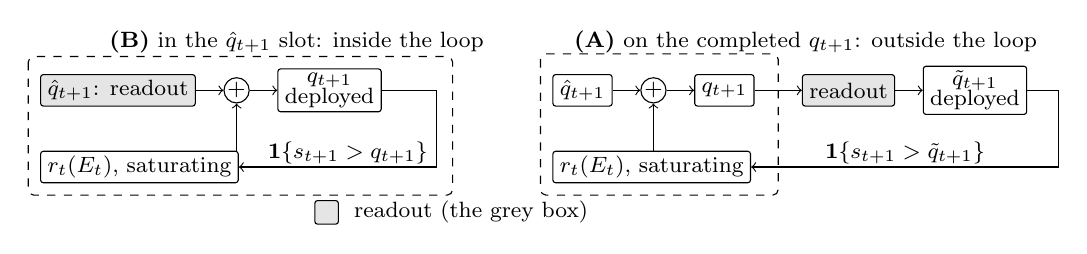
\begin{tikzpicture}[
  font=\footnotesize,
  bx/.style={draw,rounded corners=1pt,inner xsep=2.5pt,inner ysep=1.5pt,
             minimum height=4mm,align=center},
  sm/.style={bx,fill=black!10},
  jn/.style={draw,circle,inner sep=0pt,minimum size=3.2mm},
  sig/.style={->,thin},
  lab/.style={font=\footnotesize,inner sep=1pt},
  ttl/.style={font=\footnotesize,inner sep=1pt,anchor=west},
  legswatch/.style={draw,rounded corners=1pt,fill=black!10,minimum width=3mm,
             minimum height=3mm,inner sep=0pt}
]
%% ------------------------------- PANEL B -------------------------------
\begin{scope}[xshift=0mm]
  \node[ttl] at (-1.5mm,6.2mm) {\textbf{(B)} in the $\hat q_{t+1}$ slot: inside the loop};
  \node[sm]                    (Bsc)  at (0mm,0mm) {$\hat q_{t+1}$: readout};
  \node[jn,right=3.5mm of Bsc] (Bsum) {$+$};
  \node[bx,right=3.5mm of Bsum](Bq)   {$q_{t+1}$\\[-2pt]{\footnotesize deployed}};
  \node[bx,anchor=north west]  (Bint) at ([yshift=-5.6mm]Bsc.south west)
        {$r_t(E_t)$, saturating};
  \draw[sig] (Bsc) -- (Bsum);
  \draw[sig] (Bsum) -- (Bq);
  \draw[sig] (Bint.north -| Bsum) -- (Bsum);
  \coordinate (Bt) at ([xshift=7mm]Bq.east);
  \coordinate (Bc) at (Bt |- Bint.east);
  \draw[thin] (Bq.east) -- (Bt) -- (Bc);
  \draw[sig]  (Bc) -- (Bint.east) node[lab,pos=0.45,above] {$\mathbf{1}\{s_{t+1}>q_{t+1}\}$};
  \path (Bsc.west |- Bq.north)   coordinate (Bnw);
  \path (Bt       |- Bint.south) coordinate (Bse);
  \draw[dashed,thin,rounded corners=2pt]
       ([shift={(-1.5mm,1.5mm)}]Bnw) rectangle ([shift={(2mm,-1.5mm)}]Bse);
\end{scope}
%% ------------------------------- PANEL A -------------------------------
\begin{scope}[xshift=59mm]
  \node[ttl] at (-1.5mm,6.2mm) {\textbf{(A)} on the completed $q_{t+1}$: outside the loop};
  \node[bx]                    (Asc)  at (0mm,0mm) {$\hat q_{t+1}$};
  \node[jn,right=3.5mm of Asc] (Asum) {$+$};
  \node[bx,right=3.5mm of Asum](Aq)   {$q_{t+1}$};
  \node[sm,right=6mm of Aq]    (Asm)  {readout};
  \node[bx,right=3.5mm of Asm] (Aqt)  {$\tilde q_{t+1}$\\[-2pt]{\footnotesize deployed}};
  \node[bx,anchor=north west]  (Aint) at ([yshift=-5.6mm]Asc.south west)
        {$r_t(E_t)$, saturating};
  \draw[sig] (Asc) -- (Asum);
  \draw[sig] (Asum) -- (Aq);
  \draw[sig] (Aq)  -- (Asm);
  \draw[sig] (Asm) -- (Aqt);
  \draw[sig] (Aint.north -| Asum) -- (Asum);
  \coordinate (At) at ([xshift=4mm]Aqt.east);
  \coordinate (Ac) at (At |- Aint.east);
  \draw[thin] (Aqt.east) -- (At) -- (Ac);
  \draw[sig]  (Ac) -- (Aint.east) node[lab,midway,above] {$\mathbf{1}\{s_{t+1}>\tilde q_{t+1}\}$};
  \path (Asc.west |- Aqt.north)  coordinate (Anw);
  \path (Aq.east  |- Aint.south) coordinate (Ase);
  \draw[dashed,thin,rounded corners=2pt]
       ([shift={(-1.5mm,1.5mm)}]Anw) rectangle ([shift={(3mm,-1.5mm)}]Ase);
\end{scope}
%% ------------------------------- LEGEND -------------------------------
\node[legswatch] (Leg) at (26.5mm,-15.5mm) {};
\node[lab,anchor=west] at ([xshift=1.5mm]Leg.east) {readout (the grey box)};
\end{tikzpicture}
\caption{One scalar readout (grey) in its two places in~(\ref{eq:pid}); dashed is the loop $r_t$ closes. In \textbf{(B)} the loop closes on the integrator's own output, and both readouts keep $\{\hat q_t\}$ in the convex hull of $\hat q_1$ and the raw scorecaster's range, inside Corollary~2's admissible set. In \textbf{(A)} it closes on $\tilde q_{t+1}$, which it never computed, and nothing keeps the deployed sequence inside that set.}
\label{fig:placements}
\vspace{-4pt}
\end{figure}

\paragraph{One scalar, two readouts, two places.} Damping a sequentially updated scalar
has two standard readouts, both prior work. A quadratic cost gives linear partial adjustment
$\tilde{q}_{t+1} = (1-\lambda)\hat{q}^{\,\mathrm{raw}}_{t+1} +
\lambda\tilde{q}_t$ \citep{garleanu2013dynamic}, which \citet{godahewa2025stability} publish as
post-processing and \citet[Eq.~13]{binny2025whomoved} apply to a deployed conformal threshold. A
proportional cost gives a no-trade band, moving only when the
target is more than $\tau$ away, then pulling back exactly $\tau$
\citep{constantinides1986,davis1990}. Either readout has two positions in (\ref{eq:pid}), drawn
in Figure~\ref{fig:placements}. \textbf{(A)}, Placement~A, is the one measured here, and it is
the one a designer reaches for, because the deployed number is what has to sit still.
\emph{The dead band ($L_1$) is not a stylistic alternative to the partial-adjustment ($L_2$) form}; it
is the family whose failure Section~\ref{sec:forfeit} characterises. Neither is safe by construction:
$L_2$ forfeits Proposition~2's
rate while covering, $L_1$ past the radius loses coverage, and at the legal $\hat{q} \equiv
-b/2$ both lose it. So the tight quantity is the radius, not either form.

\paragraph{The quantity, and the names it already has.} We report the deployed threshold's
\emph{travel}, $\mathcal{T}_H = \sum_{t=2}^{H}|q_t-q_{t-1}|$, after actuator travel in process
control. The arithmetic is not new, and the name is a convenience rather than a contribution.
Over a predictive distribution $\sum|\Delta q|$ is the
Multi-Quantile Change \citep[v3, \S3.4.1]{zanotti2026smqc}; verification calls the same movement
\emph{jumpiness} \citep{zsoter2009jumpiness}, a \emph{convergence index}
\citep{ehret2010convergence} and forecast \emph{(in)consistency}
\citep{pappenberger2011consistency}, all three imported by \citet{vanbelle2026stabilizing};
applied control calls it IACER \citep{sarhadi2025criteria}; and dynamic-regret online learning
calls it a path length.
Section~\ref{sec:related} names ten across four vocabularies, so a fresh one is used here, for one
reading only.
% Wave 3 closed every bibliography gap in this file: zsoter2009jumpiness, ehret2010convergence,
% pappenberger2011consistency and sarhadi2025criteria (IACER, arXiv:2503.14379 eq. (6),
% criterion CR8) are all in audit/REFS_VERIFIED.bib and cited as \citep above.

\paragraph{Harness.} The harness fixes $\alpha = 0.1$ and $b = 2$. Its saturator $r_t(x) =
b\,\mathrm{clip}(x/(c\,h(t)),-1,1)$, with $c = 1$ and $h(t) = \log(t+2)$, meets~(4) with equality.
The scorecaster is null and legal, reducing (\ref{eq:pid}) to the pure error integration
Proposition~2 addresses, so the readout is the only manipulated variable. Neither choice is
neutral, and each sits at an edge of what condition~(4) and Theorem~1 allow rather than in the
middle of it: (4) is a lower bound, and this saturator meets it exactly rather than exceeding it,
while Theorem~1 permits scorecasters anywhere within $b/2$ either side of null, predictable but
not required to be constant in $t$. The adversary is specified, not
tie-broken. It plays $s_t = \mathrm{clip}(\tilde{q}_t+\varepsilon,\pm b/2)$, $\varepsilon =
10^{-9}$, against the \emph{deployed} $\tilde{q}_t$: the $\varepsilon\downarrow 0$ reading of
``sets the score at the threshold'', firing the strict indicator. Legality is Theorem~1's
$[-b/2,b/2]$ on both sides, so $b/2+b/2 = b$ is exactly tight. \emph{That specification names one
member of a class}: any adapted $s_t \in [-b/2,b/2]$ is legal, the constant $s_t \equiv -b/2$
included. Every number in Table~\ref{tab:forfeit} is measured against the
one adversary above;
Section~\ref{sec:forfeit}'s two boundaries are quantified over the class, and they differ.

% R3b, RECAST AS A TIGHTNESS RESULT.  Session S4 wave 1, agent K2.
%
% S4 WAVE 4: the li2025o2cp citation below is wrapped in \mbox BECAUSE IT MUST NOT BREAK
% ACROSS A PAGE.  pdftex cannot split a hyperref link over a page boundary -- it dies with
% "! This can't happen (pdfvlistout)" after a \pdfendlink nesting warning -- and after this
% wave's edits the page 2/3 break landed inside "Li et al. [2025, Corollary 2]".  Do not
% remove the \mbox without rebuilding and checking the page break.
%
% S4 WAVE 2 (orchestrator): the mandated L1/L2 finding sentence appeared TWICE after
% wave 1 -- K1 put it in sections/setup.tex, where L1 and L2 are defined and where the
% qhat = -b/2 clause sits in the same breath, and K2 put a second copy in the tightness
% paragraph below.  The setup.tex instance is kept and this copy is CUT.  Frees 2 body
% lines, returned to this wave's reflow budget.
%
% ORDER IS LOAD-BEARING AND IS THE WHOLE POINT OF THE REWRITE.
%   (a) li2025o2cp Corollary 2's RETENTION result is stated FIRST and belongs to
%       its authors.  It is the thing being tested, not a caveat on this paper.
%   (b) this paper exhibits ONE legal perturbation -- the L1 dead band on the
%       COMPLETED threshold -- that leaves the admissible radius, and locates the
%       edge: tau* = sup_x r_t(x) + sup_t qhat_t - b/2.
%   (c) the condition is therefore TIGHT there, i.e. NECESSARY and not merely
%       sufficient.  That is a SMALLER and MORE PRECISE claim than "smoothing
%       forfeits the rate" and it is stated without hedging against that larger
%       claim.  Elsewhere the condition stays sufficient only, and the paragraph
%       says so: that asymmetry is what makes "tight" a LOCATED claim.
%
% MOVED IN FROM sections/limitations.tex THIS WAVE.  The saturator-level-4b
% result and ACT23's tangent-integrator result sat in the concession list, where
% they read as unexplained caveats ("the headline collapses to 20.10 and nothing
% explains why").  They are the SAME mechanism as the scorecaster sweep --
% sup r_t and sup qhat are the two terms of tau* -- so they are part of the
% CHARACTERISATION and belong inside it.  limitations.tex loses those lines and
% this section gains them; the exchange is recorded in both headers.
%
% EVERY NUMBER IN THIS SECTION TRACES TO A results/ JSON (docs/GATES.md G7.1):
%   primary       results/forfeit-20260820T063045Z-83747c45.json
%   tau-cliff     results/forfeit-20260820T063132Z-83747c45.json
%   variations    results/forfeit-variations-20260820T101445Z.json
% Row-by-row trace, one row per printed number with file + JSON key path + value:
% research/S4/K2-tightness.json, field number_trace.  Code: src/forfeit.py,
% src/test_forfeit.py.
%
% S5 SUB-SESSION A (2026-08-20): NUMERIC PROVENANCE AUDIT.  All 66 Table 1 cells were
% re-derived from results/forfeit-20260820T063045Z-83747c45.json, aggregate_table, regime
% == "adversarial", and every one agrees to printed precision.  Four changes here:
%   (a) TABLE 1 GAINED "miscov. 10^6" (aggregate_table[*].miscoverage at T = 1e6), because
%       the abstract cited arm ema_w0.999's 0.100004 and the table had no 10^6 miscoverage
%       column to check it against.  Seven columns fit with 0 overfull boxes.
%       AMENDED S5 WAVE 6 (J1): THE ABSTRACT NO LONGER PRINTS 0.100004.  Wave 3's rewrite
%       dropped the 42x / T = 1e6 / 0.100004 group AS A UNIT, deliberately, so the
%       miscoverage figure could not be re-paired with the wrong horizon a second time.
%       The COLUMN stays and is right -- all eleven values re-derived twice, and it is what
%       makes the T = 1e6 arm checkable at all -- but the BOLD on 0.100004 no longer points
%       at an abstract sentence.  It is kept because the body still turns on that arm
%       (61.08 -> 42.10, travel 28,311 -> 202), i.e. it now marks what SECTION 3 discusses
%       rather than what the abstract quotes.  Recorded so nobody re-derives the reason.
%   (b) "the ratio falls with the horizon, 61.08 to 42.10" NAMED NO ARM AND NO HORIZONS, and
%       the sentence had just said "for the last two" (w = 0.99 AND w = 0.999).  61.08 and
%       42.10 are ema_w0.999 ALONE, at T = 1e4 and T = 1e6 (aggregate_table[16] and [19],
%       ratio_max_abs_E_over_bound).  Both are now named.  The flatness claim itself is
%       correct for both arms: max_abs_E is 63.00 at all four horizons for w = 0.99 and
%       623.70 at all four for w = 0.999.
%   (c) "623.70 falls to 20.10" -- 623.70 is flat in T but 20.10 is NOT (13.80/17.00/17.90/
%       20.10 across the four horizons, rows[192..195]), so the horizon is now stated.  Same
%       for the tangent tau = 1.5 miscoverage 0.100001 (rows[207]).
%   (d) "tau = 2.0, 2.5, 3.0 and 5.0 fail too" sat immediately after a T = 10^6 figure but
%       those four bands were only ever run at T = 2x10^5 (variation wide_deadbands_baseline,
%       rows[225..228]).  The horizon is now stated.
%   Also fixed: "Every dead-band dead-band configuration" -> one "dead-band".
% VERIFIED UNCHANGED, no edit needed: 70.80 is arm ema_w0.999, regime EXACT_THRESHOLD_STRICT,
% flat across all four horizons (aggregate_table[104..107].max_abs_E) -- which is exactly the
% regime the sentence describes ("playing the threshold exactly ... under the same indicator,
% because its signature move then covers").  The 6.30/63.00/623.70 triple is read off the
% actual T = 1e4 rows (aggregate_table[8], [12], [16]), not inferred from the 1e6 column.
% The 19-of-19 law check re-ran clean: 15 at T = 1e6 over five settings x three widths, plus
% 4 wide bands at T = 2e5, 0 mismatches.  "its realised supremum is b - tau to the printed
% digit at every tau >= 0.9" IS computable from results/: max(arms_raw[*].trace.q_deployed)
% equals b - tau to nine decimals at every one of the ten grid widths >= 0.9, and is 1.2203
% (< 1.5) at tau = 0.5, so the ">= 0.9" qualifier is exactly right.
%
% S4 WAVE 2 (orchestrator): TABLE 1 NOW LISTS ALL ELEVEN ARMS.  The two S3 wave 5 dropped
% to pay for the boundary-law correction -- "partial adj. w = 0.5" and "growing time
% constant p = 0.5" -- are RESTORED from results/forfeit-20260820T063045Z-83747c45.json
% (aggregate_table, arms ema_w0.5 and growing_ema_p0.5, regime adversarial, T = 2e5 and
% 1e6).  Both cover and both sit inside the bound, so restoring them removes a disclosure
% caveat rather than adding evidence.  Prose counts updated nine -> eleven.  Also restored,
% because the resize freed the space K2 had to compress them into: the T = 10^4 excursion
% triple, the anti-windup mechanism sentence, and the tie-rule sentence.
%
% SUPERSEDED NOTE, kept for the record:
% TABLE 1 LISTS NINE OF THE ELEVEN ARMS RUN.  "partial adj. w = 0.5" (0.100030,
% 7.70, 0.52, 0.0000, 18,113) and "growing time constant p = 0.5" (0.100030,
% 12.60, 0.85, 0.0000, 330) were dropped in S3 wave 5 to pay for the boundary-law
% correction.  Both COVER and both sit inside the bound, so nothing adverse is
% hidden; every count in the prose is stated against the nine that are listed.
% The table is UNCHANGED this wave.
%
% WAVE-5 CORRECTION, CARRIED (S3 F1, research/S3/F1-adversarial.json 0-4).  An
% earlier version printed "coverage survives if and only if tau <= b/2" and "the
% failing set is (b/2,b]".  Both are false as general statements.  b/2 is the
% value of tau* at the NULL scorecaster and the MINIMAL admissible saturator; a
% legal constant scorecaster moves it, and the failing set is unbounded above.
%
% S4 CORRECTION, G7.1: "coverage survives to tau = b" IS DELETED.  It was printed
% of the qhat = +b/2 arm, where tau* = b, but no dead band of width b was ever RUN
% at that scorecaster -- the widths run there are 0.5, 0.9 and 1.5.  The sentence
% was a prediction from the law wearing the clothes of a measurement.  Replaced by
% the measurement: every width run at +b/2 covers, tau = 1.5 at 0.100010.
%
% S4 CORRECTION, G7.1: "31 OF 32 GRID POINTS" IS NOT PRINTED.  docs/GATES.md
% G7.9, docs/OUTSTANDING.md O52 and docs/S3_REPORT.md sec. 2 all carry it, and
% all three rest on ONE line in research/S3/patch-log.json -- an S3 orchestrator
% assertion in a gitignored file.  Neither the 32 points nor the unresolved one is
% identified anywhere, and no 32-point grid is reconstructible from results/.  A
% number that cannot be traced is deleted, not footnoted.
%
% WHAT IS PRINTED INSTEAD, AND IT IS FULLY TRACEABLE.  Applying tau* = sup_x
% r_t(x) + sup_t qhat_t - b/2 (b = 2, and sup_x r_t(x) = saturator_level_mult * b
% by src/forfeit.py:306) to every dead-band configuration in
% results/forfeit-variations-20260820T101445Z.json and comparing the predicted
% verdict with the measured miscoverage: 15/15 at T = 10^6 over the five
% (saturator, scorecaster) settings (baseline, qhat = +b/2, qhat = -b/2, level 4b,
% ACT23 tangent) at tau = 0.5/0.9/1.5, plus 4/4 on the wide bands tau =
% 2/2.5/3/5 at T = 2e5 -- 19 OF 19, NO COUNTEREXAMPLE.  Verified independently by
% K2; the arithmetic is in research/S4/K2-tightness.json (law_check_19_of_19).
% results/forfeit-20260820T063132Z-83747c45.json adds 11 more widths at the
% baseline setting, also 11/11, and is NOT folded into the printed count.
% The resolution caveat -- three widths per setting bracket each edge rather than
% locate it -- and the run that would close it are printed in the same sentence.
%
% FRAMING sec. 3: every quantifier is a measurement; no forbidden construction.
% The endpoint COVERS, so "tau > tau*" is the failing condition and writing
% "tau >= tau*" would be wrong.

\section{The edge of the admissible set, measured}
\label{sec:forfeit}

\begin{table}[tb]
\centering
\scriptsize
\setlength{\tabcolsep}{4.5pt}
% S5 wave 4: arraystretch 0.95.  Eleven data rows at 0.95 give back one typeset line,
% which was two of the last two lines standing between the body and the 4-page ceiling.
% This is row LEADING only -- no font change, no row removed, no cell altered.
\renewcommand{\arraystretch}{0.95}
% S6 SUB-SESSION B: CAPTION REWRITTEN TO DESCRIBE ONLY.  Two clauses left, and neither
% was deleted:
%   "so no covering arm is withheld" was a REBUTTAL, not a description.  The fact it
%     defended -- that every arm run appears -- is still the caption's first sentence.
%   "five exceed the bound at T = 10^6" was a CONCLUSION about the data, and it existed
%     NOWHERE ELSE in the paper (grepped: one hit, this caption).  It moved into the
%     retention paragraph below, where Table 1 is first discussed.  Independently
%     recounted from the table's own ratio column: 4.25, 42.10, 3.58, 3.34 and 60,747
%     exceed 1, so five is right.
\caption{Placement~A: a one-scalar readout on the \emph{completed} threshold, under one
deterministic adversary, on one pass to $T = 10^6$; all eleven arms run are listed.
Proposition~2's bound is $13.2061$ at $T = 2{\times}10^5$ and $14.8155$ at $T = 10^6$;
``ratio'' is $\max_t|E_t|$ over it, and ``Sat.'' the fraction of rounds on which~(4)
delivers its full $\pm b$. Every number is the \emph{primary} regime's, defined in
Appendix~\ref{app:support}, which also gives the $T = 10^4$ excursions and the fitted
excursion law.}
\label{tab:forfeit}
\begin{tabular}{@{}lrrrrrr@{}}
\toprule
Readout on the completed threshold & miscov.\ $2{\times}10^5$ & miscov.\ $10^6$ &
$\max_t|E_t|$ $10^6$ & ratio & Sat.\ $10^6$ & travel $10^6$ \\
\midrule
none (control)                & $0.100035$ & $0.100007$ & $7.80$        & $0.53$     & $0.0000$ & $28{,}311$ \\
partial adj.\ $w = 0.5$       & $0.100030$ & $0.100007$ & $7.70$        & $0.52$     & $0.0000$ & $18{,}113$ \\
partial adj.\ $w = 0.9$       & $0.100030$ & $0.100007$ & $7.50$        & $0.51$     & $0.0000$ & $4{,}081$ \\
partial adj.\ $w = 0.99$      & $0.100040$ & $0.100006$ & $63.00$       & $4.25$     & $0.0007$ & $1{,}023$ \\
partial adj.\ $w = 0.999$     & $0.100035$ & $\mathbf{0.100004}$ & $623.70$      & $42.10$    & $0.0097$ & $202$ \\
growing time constant $p=0.5$ & $0.100030$ & $0.100006$ & $12.60$       & $0.85$     & $0.0000$ & $330$ \\
growing time constant $p=0.9$ & $0.100030$ & $0.100024$ & $53.00$       & $3.58$     & $0.3181$ & $16$ \\
running mean                  & $0.099940$ & $0.100010$ & $49.50$       & $3.34$     & $0.3647$ & $9$ \\
dead band $\tau = 0.5$        & $0.100035$ & $0.100005$ & $10.60$       & $0.72$     & $0.0000$ & $2{,}045$ \\
dead band $\tau = 0.9$        & $0.100060$ & $0.100012$ & $13.20$       & $0.89$     & $0.0038$ & $1{,}051$ \\
dead band $\tau = 1.5$        & $\mathbf{1.000000}$ & $\mathbf{1.000000}$ & $900{,}000$ & $60{,}747$ & $1.0000$ & $0.5$ \\
\bottomrule
\end{tabular}
\end{table}

\paragraph{The retention result is published, and tested from outside.}
\mbox{\citet[Corollary~2]{li2025o2cp}} prove that a predictable $d_t$ with $|d_t| \le
\mu_t(b/2-|\hat{q}_t|)$ on the deployed threshold keeps (\ref{eq:pid}) in error-integration form
and \emph{retains} $|E_T| \le c\,h(T)+1$: the radius is theirs. A downstream partial
adjustment of weight $w$ leaves it; Table~\ref{tab:forfeit} prices that departure, and five of its
eleven arms exceed the bound at $T = 10^6$. For $w = 0.99$ and
$0.999$ the excursion is \emph{flat in $T$} while the bound grows like $\log T$. At $w = 0.999$
the ratio is $61.08$ at $T = 10^4$ and $42.10$ at $T = 10^6$. The
forfeit is a property of the smoothing \emph{strength}, not Placement~A, and it buys something:
travel falls from $28{,}311$ to $202$. The forfeit's sign is counter-intuitive. A readout on the completed
$q_{t+1}$ touches neither $r_t$ nor the integrator's argument, so it cannot put~(4) at risk. It delays a
correction already computed, and the accumulator excurses
\emph{further}. Smoothing the output does not damp $E_t$; it feeds it. That $623.70$ turns on the
adversary's $\varepsilon$, not the counting convention.

% ---------------------------------------------------------------------------
% S5 WAVE 2: sub-session B's boundary figure, inserted here.
% It is referenced by \ref{fig:boundary} from the paragraph immediately below.  It
% appears AFTER the schematic in document order, so LaTeX typesets it as Figure 2.
%
% S6 SUB-SESSION A: REBUILT.  Two measured defects drove it, both recorded in
% research/S6/A0-diagnosis.json and both re-measured against the RENDERED artefact
% rather than read off the generator:
%   (1) the old panel (b) placed the eleven-point grid by INDEX.  The located window
%       tau in [1, 1.001] took 10.000% of that axis while being 0.0910% of the true log
%       span: inflated x109.9, which erased the one thing the grid was run to show.  It
%       is now placed by tau - tau* on matplotlib's native SYMLOG scale, linthresh 1e-3.
%   (2) panel (a) carried five settings, five tau* markers in three styles, two inline
%       annotations and a legend.  Four markers nested at (tau=0.5, miscov~0.1) and the
%       legend frame overwrote 627 px of the tau*=1 rule and 651 px of the tau*=2 rule
%       (pixel diff, legend drawn vs not drawn, 400 dpi).  Panel (a) now carries ONE
%       setting: the null scorecaster, the only one with runs on both sides of its own
%       tau*.  The five-setting comparison moved to Figure~\ref{fig:settings} in
%       Appendix~\ref{app:support}, where a categorical axis can do it properly.
% NOT A DEFECT, recorded because the S6 brief asserted it was one: panel (a)'s x-axis was
% ALREADY log-scaled under S5.  Its rendered tick positions matched true log positions to
% 1.1e-16 and the gap-by-gap distortion factor was exactly 1.000 at all six gaps.
%
% Built by src/make_figure1.py, which reads results/ directly and whose check_law() and
% check_grid_law() re-derive tau* per setting and test it against every measured
% miscoverage, exiting non-zero on any inconsistency -- so neither figure can be produced
% from data that contradicts the law it draws.  Its overlap_audit() then fails the build
% on any two text or legend boxes that come within 1.6pt of each other.  The generator
% pins CreationDate, so re-running it reproduces both PDFs byte for byte.
% THE CAPTION CARRIES NO EM-DASH.
% ---------------------------------------------------------------------------
\begin{figure}[tb]
  \centering
  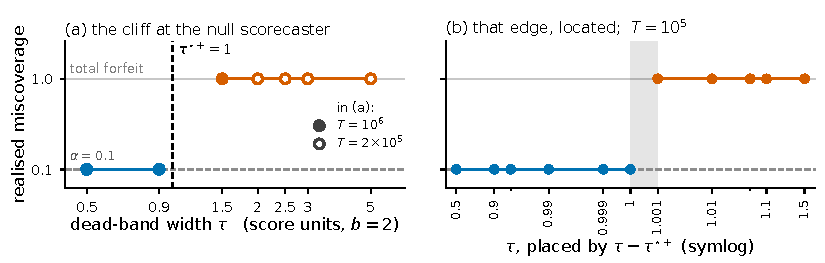
\includegraphics[width=\textwidth]{figures/figure1_boundary.pdf}
  \caption{Realised miscoverage against dead-band width $\tau$ at the null scorecaster,
  $\hat{q} \equiv 0$ with a saturator of level $b$, where $\tau^{\star} = \sup_x r_t(x) +
  \sup_t \hat{q}_t - b/2$ is $1$. \textbf{(a)} The full sweep: filled markers run to
  $T = 10^{6}$ and the four widest bands, drawn open, to $T = 2{\times}10^{5}$; blue
  covers, orange forfeits, and the dashed rule is $\tau^{\star}$. \textbf{(b)} The same
  setting at $T = 10^{5}$ over eleven measured widths, placed by $\tau - \tau^{\star}$ on
  a symlog axis whose linear zone is $|\tau - \tau^{\star}| \le 10^{-3}$, which magnifies the
  neighbourhood of $\tau^{\star}$: visual spacing here is not proportional to true distance in
  $\tau$. Unlabelled minor ticks mark $\tau = 0.95$ and $1.05$. The grey band spans the widest covering width to the
  narrowest failing one; Figure~\ref{fig:settings} gives the other four $(r_t,\hat{q})$
  settings.}
  \label{fig:boundary}
\end{figure}

\paragraph{The $L_1$ dead band leaves the radius, and the edge is measurable.} A dead band pulls
the deployed threshold back by exactly $\tau$ when it releases, so ``inside Corollary~2'' reads
$\tau \le \mu_t(b/2-|\hat{q}_t|)$. Under saturation the deployed value is pinned $\tau$ below the
integrator's ceiling, and its realised supremum is $b-\tau$ to the printed digit at every $\tau \ge
0.9$. The adversary's best legal play is $b/2$, so coverage is lost when that supremum drops below
it, at $\tau^{\star} = \sup_x r_t(x) + \sup_t \hat{q}_t - b/2$. All $19$ dead-band
runs agree with that law (Figure~\ref{fig:settings}); only the null scorecaster's edge is located
(Figure~\ref{fig:boundary}), the others one-sided. \textbf{Here $\sup_x r_t(x) = b$ and $\hat{q} \equiv 0$, so
$\tau^{\star} = b/2$}, one point of the admissible class, and both terms move it. The legal
$\hat{q} \equiv +b/2$ carries the $\tau = 1.5$ band inside the bound. The equally legal $\hat{q}
\equiv -b/2$ drops the edge to $0$, and there $\tau = 0.5$ returns $1.000000$, as does partial
adjustment at $w = 0.999$. Condition~(4) bounds $\sup_x r_t(x)$ only from below, so raising it
costs the theorem nothing; it moves the edge too (Figure~\ref{fig:settings}) and shrinks
the excursion. Under the unbounded tangent integrator
\citet{angelopoulos2023pid} report using in all their experiments, $\tau^{\star}$ is unbounded and
all three widths there cover. The excursion is $20.10$ rather than $623.70$, both at $T = 10^6$. \textbf{The method's own integrator therefore
sits inside the set at every width run here.} Outside the set the transition is a step. Past
$\tau^{\star}$ the threshold sits permanently below the reachable score range and $|E_t| =
(1-\alpha)t$ grows linearly, $60{,}747$ times the bound at $T = 10^6$. The wider bands $\tau =
2.0$, $2.5$, $3.0$ and $5.0$ fail too at $T = 2{\times}10^5$ (Figure~\ref{fig:boundary}), so the
failing set is $(\tau^{\star},\infty)$, open at the left. \textbf{The endpoint is where the adversary's
specification decides the answer.} At $\tau = \tau^{\star}$ the deployed supremum equals the
adversary's own cap $b/2$, so the clip forces an exact play and the reading settles it: the
primary regime covers. Appendix~\ref{app:support} separates the two readings and prints both.
\textbf{The failing arms have $\mathrm{Sat.} = 1.0000$.} Condition~(4) delivers its full
$\pm b$ on every round, and what fails is Proposition~2's other hypothesis: the threshold closing
the loop \emph{is} the integrator's output.

\paragraph{What that measures is that the published condition is tight.} At $\mu_t = 1$,
$\hat{q} \equiv 0$ the measured $\tau^{\star}$ is exactly Corollary~2's radius, and crossing it
costs coverage rather than the rate. \textbf{The claim is that necessity: a tightness result about
someone else's sufficient condition}, smaller and more precise than a forfeit of the rate by
post-processing. Elsewhere it stays sufficient only: at $\hat{q} \equiv +b/2$ Corollary~2
permits radius $0$ while every width run there covers. That asymmetry makes ``tight'' a located
claim.

\paragraph{The constructive reading, and it is the corollary's rather than ours.} Placement~B
keeps $\{\hat{q}_t\}$ inside the admissible radius, so Theorem~1 carries it already. What the
measurement adds is that the band has an edge, computable before deployment from $\sup_x r_t(x)$
and $\sup_t \hat{q}_t$, and that crossing it is not a graceful degradation.

% Related work.  SESSION S4 WAVE 1, AGENT K3: R3c IS DEMOTED TO DESCRIPTIVE RELATED
% WORK AND IS NOT A CONTRIBUTION.  docs/FRAMING.md sec. 2.2c records that S3's own
% H6 agent falsified the four-literature disconnection -- Semantic Scholar's
% citations endpoint for kalai2005lazy returns 875 citing works, three of them
% online conformal, one of them chen2023ipoc, which this paper already cites.  The
% payload never needed the disconnection and is what survives here: four
% vocabularies name one quantity, and this paper's object sits in one of them.
%
% WHAT WAS DELETED THIS WAVE.  All of it was the machinery of a claim the paper no
% longer makes.
%   (a) Table 2's "Cites the other three?" row -- 0/437, 1/437, 0/437; 1/226,
%       8/226, 3/226; 0/106; 0/93.  A cross-citation census is evidence for or
%       against a disconnection; with no disconnection claimed it supports nothing,
%       and printed counts invite the reading the paper disowns.
%   (b) Table 2's "Lacks that the others have" row.  A four-way comparative claim
%       of ABSENCE, and three of its four cells were quantifiers ("any interval or
%       coverage object", "a decision that pays to move", "a calendar-time path
%       functional") rather than instrument-scoped counts.
%   (c) The whole cross-citation paragraph: the 862 references, the 13 crossings,
%       the "concentrated rather than sparse" gloss, the over-matching-index
%       caveat, the bolded "We claim no disconnection", and the 875-citing-works
%       refutation.  A printed denial of a claim the paper does not make is the
%       last residue of the contribution: it tells a referee to look for a bridge
%       claim that is not there.
%   (d) The caption's closing cross-citation sentence, which sourced (a).
% The surviving row is renamed from "Has that the others lack" -- itself a
% comparative absence claim -- to a plain statement of what each field contributes.
%
% KEPT DELIBERATELY.
%   - The caption names TEN names across FOUR vocabularies and is load-bearing:
%     sections/setup.tex cites this caption for that count, because docs/GATES.md
%     G7.11 requires the names to be conceded and the total NOT to be printed.
%   - "What is conceded, by name" is untouched in substance.  It carries G7.4's
%     concession list (placement -> ACT23 / Dupuy / Duerst; derivation ->
%     li2025o2cp Cor. 2 and wang2026acmcp; smoother object, metric arithmetic and
%     both readout forms -> sections/setup.tex; anti-windup -> galeani2009antiwindup)
%     and G7.5's concession of the derivation by name.
%   - ANDREW ET AL. THEOREM 7 STAYS PRINTED AS THE TRADE-OFF IT IS (docs/FRAMING.md
%     sec. 3, corrected 2026-08-20): sublinear regret is bought by growing theta
%     with T, which grows the competitive ratio.
%
% Every \citep key below resolves against audit/REFS_VERIFIED.bib.  Four keys this
% file used to cite are now cited by no file: zinkevich2003ogd, kalai2005lazy,
% zhang2024bayesianocp, ramalingam2025noregret.  They stay in the .bib and plainnat
% prints only cited entries, so nothing breaks; they are reported to the
% orchestrator in research/S4/K3-demotion.json.
%
% DOWNSTREAM, REPORTED AS A HANDOFF (K3 does not own that file):
% sections/limitations.tex still reads "Seven of the twenty-six anchors return an
% empty reference list, so Table 2's counts are gaps rather than zeros."  Table 2
% no longer prints counts, so that sentence is orphaned and should be cut.
%
% S5 SUB-SESSION G3 (2026-08-20): PROSE AND PUNCTUATION PASS.  No concession was
% dropped, softened or renamed; every \cite key that was here is still here, and
% Table 2 (caption, row, and the Andrew et al. Thm 7 TRADE-OFF wording) is
% untouched.  What changed:
%   (a) BOTH EM-DASHES ARE GONE.  The pair around "the admissible set around the
%       deployed threshold" was a genuinely subordinate appositive, so it is now
%       parenthesised.  File em-dash count 2 -> 0.
%   (b) TOPIC SENTENCE PER CONCESSION.  The run-on enumeration is now one short
%       declarative sentence per concession: placement / derivation / Section 2's
%       objects / the four smoother-in-the-argument papers / anti-windup /
%       gao2025coloke.  No sentence exceeds 28 words; the longest before was 45.
%   (c) TWO CITATIONS MOVED TO THEIR natbib LOCATOR FORM, which prints the same
%       information in fewer characters: \citet[Appendix~A]{dupuy2026relevance}
%       and \citet[Corollary~2]{li2025o2cp}.  The second replaces a
%       \citeauthor{...}'s Corollary~2 ... \citep{...} pair that named li2025o2cp
%       twice.  G7.5 still reads on it: "Li et al. [2025, Corollary 2]" names the
%       derivation's prior art in the printed text.
%   (d) THE OPENING SENTENCE IS NOW RUN INTO THE CONCESSION PARAGRAPH and the
%       \paragraph head is a \textbf run-in lead, which is the style
%       sections/limitations.tex already uses.  THIS IS THE ONLY STRUCTURAL
%       CHANGE AND IT IS WORTH EXACTLY ONE TYPESET LINE: the standalone opening
%       paragraph ended a line 45 characters short, and merging recovers it.
%       Reverting it (restore \paragraph{What is conceded, by name.} and the
%       blank line) costs one line and nothing else.
% MEASURED, three passes + bibtex: section 4 spanned margin lines 136-152 (17
% typeset lines) before, 131-145 (15) after.  2 lines saved.  0 undefined
% citations, 0 overfull boxes, 0 \pdfendlink warnings.

% S5 WAVE 6, J1 FINDING 4: AN UNSUPPORTED CLAIM ABOUT OUR OWN MEASUREMENT IS DELETED.
% This paragraph used to end "Section 3 measures that accumulation diverging", of
% gao2025coloke's assumption that sum_{t<=T} q_t <= O(alpha h(T)).  SECTION 3 MEASURES NO
% SUCH THING.  No results/ field holds sum_t q_t: aggregate_table carries max_abs_E and
% deployed_travel, and travel is sum|delta q|, a DIFFERENT quantity.  Worse, the mean
% deployed threshold is about +1.06 for the UNSMOOTHED control, so the sum the sentence
% pointed at grows linearly for this paper's own baseline too -- cashed out, the sentence
% indicted a neighbour's assumption on a ground our own control also violates.
% G7.1's standard is that an untraceable claim is deleted rather than footnoted, so it is
% deleted.  What survives is the accurate part: their assumption is supported with a plot
% rather than derived, which is their own Fig. 2a caption's wording.

% S8 SUB-SESSION D (2026-08-22): OPENING POINTER TRIMMED, NOT RESTRUCTURED.  This
% session verified the four-vocabularies material is NOT duplicated in the body -- this
% opening is already just a two-sentence pointer at Table~\ref{tab:bridge} in
% Appendix~\ref{app:bridge}, and the concession paragraph that follows is separate
% content already conceding by name, not a restatement of the table.  Cut, each because
% it is redundant with material established elsewhere rather than because it is
% unwanted: "many ways" (filler); "the object that settles its validity" and "around the
% deployed threshold" (both glossing what the admissible set is, which sections/setup.tex
% already establishes -- see its Fig.~2 caption and "The quantity, and the names it
% already has"); and "and what each contributes" (the table's own caption already says
% "The row gives what each contributes"); and "the object that settles its validity
% ... sits in the first of them" (the claim that the admissible set is specifically the
% first of the four vocabularies -- also redundant with setup.tex's framing, and
% recoverable from Table~\ref{tab:bridge}'s own first row rather than asserted twice).
% CORRECTED 2026-08-22 (S8-F adversarial critic caught this comment overstating what
% survived): what actually remains is ONE clause, not a sentence pair -- that four
% vocabularies name one quantity, and a pointer to Table~\ref{tab:bridge} that still
% names the appendix explicitly (App.~\ref{app:bridge}) rather than relying on the
% reader to follow the cross-reference blind. The admissible-set-is-first claim is not
% restated in body prose; it is still readable off the table's own first row, which is
% why the cut is defensible -- but the prior wording here was wrong to say that clause
% survived in prose.
%
% MEASURED AGAINST THE 4-PAGE CEILING, AND REPORTED HONESTLY.  sub-session C's own
% concurrent edits to sections/limitations.tex (the seed/determinism split, out of scope
% here) added roughly two typeset lines back to this same page.  This paragraph and the
% Introduction's four-surface sentence (sections/intro.tex) are the two compressions this
% session was authorised to make.  Isolated A/B rebuilds (reverting each file to its
% pre-S8 baseline one at a time, holding the other fixed) showed the Introduction's cut
% does not reach this page at all -- Figure~1's placement absorbs it two pages upstream --
% while THIS paragraph, once trimmed this far, recovers exactly one typeset line on the
% page the spill is on. That closes one of the body's two spilling lines. The second
% spilling line survives after this paragraph is cut to its bridging-pointer minimum;
% no further reduction here is a compression rather than a deletion, and the two
% authorised categories are now exhausted. See sections/intro.tex's matching note and
% research/S8/D-compression.json for the measured before/after and the honest verdict.
%
% S10 SUB-SESSION A (2026-08-22): THE E-VALUE / ANYTIME-VALID BRIDGE PARAGRAPH IS ADDED HERE,
% AT THE END OF THIS SECTION, AND NOWHERE ELSE.  The venue is E-values, and E_t is a running
% sum of centred miscoverage indicators, which is one transform from that venue's own object.
% It goes here rather than in sections/intro.tex because this section is the paper's
% positioning section and the Introduction's hook-then-two-claims structure (S6 sub-session C)
% has no slot for a third register before the claims are stated.
%
% WHAT LEVEL OF CONNECTION IS CLAIMED, AND WHY THAT LEVEL.  A STRUCTURAL CORRESPONDENCE THAT
% BECOMES FORMAL ONLY AFTER THE STANDARD EXPONENTIAL TRANSFORM -- NOT A SPECIAL CASE, AND NOT
% AN ANYTIME-VALID GUARANTEE.  The paragraph states three things and no fourth:
%   (1) TRUE AND EXACT, no hedge needed.  In the Shafer-Vovk protocol, a Skeptic who pays
%       alpha each round for the payoff err_t has cumulative net gain sum_{i<=t}(err_i - alpha)
%       = E_t.  That is an identity, not an analogy, and it needs no probability measure --
%       which is why it survives on this paper's adversarial paths.
%   (2) EXPLICITLY DENIED.  E_t is NOT an e-value and NOT an e-process.  Vovk and Wang's
%       definition is a NONNEGATIVE variable with expectation at most 1 under a null; E_t is
%       signed, is unbounded below, and has no null attached -- Conformal PID's Proposition 2
%       is a PATHWISE bound obtained by feedback (the saturating integrator forces it), not a
%       probabilistic statement obtained from Ville's inequality.  Claiming otherwise at an
%       e-values venue would be the single most scrutinised sentence in the paper, so the
%       paragraph denies it in its second sentence rather than leaving it to be inferred.
%   (3) TRUE, AND THE ONLY FORMAL PART.  Under the null err_t | F_{t-1} ~ Bernoulli(alpha),
%       M_t = prod (1 + lambda(err_i - alpha)) is a test martingale for lambda in
%       [-1/(1-alpha), 1/alpha] (nonnegative by that range, M_0 = 1, exactly a martingale
%       since E[err_i - alpha | F_{i-1}] = 0), and log(1+x) = x + O(x^2) gives
%       log M_t = lambda E_t + O(lambda^2 t).  So the paper's accumulator is the FIRST-ORDER
%       LOG of a test martingale, which is a real correspondence and is all of one.
% WHY S9's IFF THEOREM MAKES THIS STATEABLE (brief point 3, answered YES).  The transferred
% statement is about the GROWTH RATE of |E_T| across a whole class, not about one setting: on
% the retention side |E_T| <= c h(T) + 1 = O(log T), so log M_T = lambda O(log T) -
% Theta(lambda^2 T) -> -infty and every nonzero fixed stake is wiped out; on the failure side
% |E_T| = (1-alpha)T or alpha T, so a fixed lambda of the right sign grows M_T exponentially
% and a Ville-based test rejects at any fixed level in O(1) rounds.  A single measured
% miscoverage figure would have licensed neither half: it says nothing about the other
% adversaries in the class and nothing about the growth rate.  Because S9 proved the boundary
% two-sidedly IN |E_T| rather than in the miscoverage rate, the e-process reading inherits the
% dichotomy for free, and the paragraph says "proved in both directions" for exactly that
% reason.  This also matches the paper's own line that "the failure criterion is |E_T|, not
% the miscoverage rate" (sections/forfeit.tex).
% NOT TOUCHED, and out of scope by the brief: R3a's substance, and the open band
% sigma^+ < tau <= tau^{star+} for a genuinely time-varying scorecaster.  The paragraph's
% dichotomy is asserted only where the theorem is two-sided, i.e. on the same sub-class
% Section 3 states it for.
% CITATIONS.  Three new keys, all fetched and read this sub-session and all recorded with
% Crossref/Project Euclid metadata in audit/REFS_VERIFIED.bib's S10 block: shafer2019gtfpf
% (the protocol), ramdas2023savi (test martingale / e-process / Ville, and the existing
% game-theoretic work on testing forecaster CALIBRATION, which is why the reading is offered
% as available rather than as new), vovk2021evalues (the definition E_t fails).  One key was
% ALREADY IN THE .bib AND UNCITED and is now cited: podkopaev2024betting -- the nearest
% neighbour, and the paragraph distinguishes it correctly, since its betting is
% Orabona-Pal coin betting used as a PARAMETER-FREE OPTIMISER for the threshold, not a test
% martingale used as evidence.  Record: research/S10/A-evalue-bridge.json.
% S10 SUB-SESSION D (2026-08-22): THIS FILE MOVED OUT OF THE BODY, WHOLE AND UNCUT.
% main.tex no longer \inputs it between sections/forfeit.tex and sections/limitations.tex;
% it is \input AFTER sections/appendix.tex, so \appendix is already in force and this
% renders as Appendix~C.  NOT ONE WORD OF EITHER PARAGRAPH IS CHANGED -- the concession
% list and sub-session A's e-value / anytime-valid bridge paragraph are byte-identical to
% what they were at HEAD 5a8019e, including the explicit denial that E_t is an e-process.
% WHY: the E-values ceiling is 4 body pages "excluding references and optional appendices",
% and after S9's theorem and S10's two additions the body measured 5.934 pages.  This
% section is the largest block in the body that is not a result, and moving it is a
% RELOCATION, not a cut: the section is still in the PDF, still numbered, still findable in
% the outline, and sections/intro.tex's closing roadmap sentence now points at it by name
% and names the game-theoretic reading so a reader at an e-values venue meets it in the
% body.  \label{sec:related} is unchanged, so that pointer resolves automatically.
% REVERTING IS ONE LINE EACH WAY: move the \input back above % Limitations.  A concession list, deliberately not softened; run-in bold leads
%
% S4 WAVE 2 (orchestrator): three additions, paid for by the space the R3c demotion freed
% -- Placement B restated as CONCEDED rather than unrepaired, the single-seed and
% bracket-not-bisect caveats made explicit, and a falsification condition printed. The
% section was 11 typeset lines after wave 1, which is thin for a paper making a necessity
% claim.
% rather than \paragraph blocks to save vertical space in a 4-page body.  Every
% item is either something a referee would otherwise find, or something this
% project's own audit already found.  The R1 items (market model, position map,
% Kelly, transaction costs, turnover, basis points, net log growth, the Ryan
% replication and the measurement-leg occupancy) are DELETED, not compressed: the
% claim they belonged to is gone.
%
% SESSION S4 WAVE 1, AGENT K2.  FOUR CUTS AND ONE MOVE, all recorded here.
%
% MOVED OUT, to sections/forfeit.tex: the saturator-level-4b result (623.70 ->
% 120.60) and ACT23's tangent-integrator result (tau = 1.5 covers at 0.100001,
% 623.70 -> 20.10).  Here they read as unexplained caveats on the headline.  They
% are the SAME mechanism as the scorecaster sweep -- sup r_t and sup qhat are the
% two terms of tau* -- so they belong in the characterisation, where raising
% sup r_t is shown to raise the edge.  The lines this file loses pay for the lines
% forfeit.tex gains; see that file's header for the other half of the exchange.
%
% CUT 1, G7.1, UNTRACEABLE NUMBER.  "under the tangent 0.100025" is DELETED.  It
% is the i.i.d. control under the tangent integrator and it lives in
% research/S3/f1_probe_iid.json (key iid_tangent_null[1].miscoverage), which was
% never booked into results/.  The only 0.100025 anywhere in results/ belongs to a
% different arm entirely (variations, scorecaster +b/2, dead band tau = 0.9,
% T = 2e5).  G7.1: a number that cannot be traced is deleted, not footnoted.
%
% CUT 2, G7.1, UNTRACEABLE NUMBER.  "[0.821,0.979] at T = 2500" is DELETED, and
% docs/OUTSTANDING.md O56 -- "the one untraced number in the body" -- is thereby
% discharged by deletion rather than by sourcing.  S3's own F1 reproduced the
% interval to four decimals but ONLY after supplying two constants the paper does
% not state (K_I = b/2, and a delta with ceil(log(2500)delta) = 1), and it is
% sensitive to both: K_I = b gives [0.844,0.956] and delta = 0.2 gives
% [0.731,1.069].  T = 2500 appears nowhere in ACT23.  What survives is the RATE,
% which is derivable from the printed formula (c h(T)+1)/T at h(t) = t/log t and
% needs no constant: the certificate decays as O(1/log T), not O(1/T).
%
% CUT 3, ORPHANED BY K3.  "Seven of the twenty-six anchors return an empty
% reference list, so Table 2's counts are gaps rather than zeros" is DELETED.
% sections/related.tex no longer prints cross-citation counts, so the caveat had
% nothing left to qualify.  This is K3's handoff, accepted.
%
% CUT 4, FRAMING sec. 3 WATCH-LIST.  "a blind rerun" -> "a rerun done without
% sight of them", and "No downstream readout here recovers the bound" -> a scope
% statement naming Placement B.  Both were quantifiers standing in for
% measurements; neither word is load-bearing and both are cheap to retire.
%
% CUT 5, G7.1, ADDED MID-WAVE ON THE ORCHESTRATOR'S TRACE (research/S4/grid-trace.md).
% An earlier draft of this file conceded "one grid point of the thirty-two checked
% reached the record as a count rather than by name".  "31 of 32" does not trace to
% any committed artefact -- it rests on one line of a gitignored S3 file -- so it is
% not printed at all, here or in forfeit.tex, and the concession that referred to it
% goes with it.  What forfeit.tex prints instead is the traceable 19-of-19 check and
% its resolution caveat.

% S5 SUB-SESSION A (2026-08-20): "under i.i.d. scores it returns 0.249376" NOW NAMES ITS
% HORIZON.  The figure is aggregate_table[163].miscoverage -- arm deadband_tau1.5, regime
% iid, T = 10^6 -- and that arm's i.i.d. miscoverage moves with T (0.244700 / 0.250440 /
% 0.250515 / 0.249376), so an unqualified number was ambiguous.  The framing is honest: with
% n = T = 1,000,000 and p = 0.25, se = sqrt(p(1-p)/n) = 0.000433, and 0.249376 sits 1.44
% standard errors below 0.25 -- ordinary sampling noise around the exact value the uniform
% -score calculation predicts, not a discrepancy.  n_err = 249,376 is stored alongside it.

% S5 SUB-SESSION G3 (2026-08-20): PROSE AND PUNCTUATION PASS.  EVERY CONCESSION
% SURVIVES, including the horizon qualifier "at T = 10^6" that sub-session A
% added, the O(1/log T) rate, the absolute dead-band widths, the rebuilt-harness
% admission, Placement B, the single seed with only the null scorecaster's edge
% located, and the falsification condition.  Nothing was cut for space.
%   (a) THE ONE EM-DASH IS GONE.  "...confirmation of the mechanism --- the
%       threshold pins at..." joined two independent clauses, so it is now a
%       sentence break.  File em-dash count 1 -> 0.
%   (b) THE FIRST BOLD LEAD IS NOW A SENTENCE.  "One construction, one adversary,
%       one saturator, and 0.63/(1-w) is specific to..." had a nominal fragment
%       joined by "and" to a clause.  "The evidence is one construction, one
%       adversary, one saturator" keeps the concession word for word and makes
%       the paragraph open on a plain claim.
%   (c) "Under the tangent integrator h(t) = t/log t, SO the certified gap..."
%       was ungrammatical; the "so" is dropped and the sentence split at the
%       rate, which also brings both halves under the number-density rule.
%   (d) THREE OTHER SENTENCES SPLIT so that none carries more than two numeric
%       claims: the b = 2 conversion, the i.i.d. return at its horizon, and the
%       pin-plus-uniform-score explanation are now three sentences, not one.
% MEASURED, three passes + bibtex: the section spanned margin lines 153-165 (13
% typeset lines) before and 146-158 (13) after.  It saved nothing and it was not
% expected to: after wave 2 every line but the last was 91-106 characters full,
% so there is no slack here that is not content.  The 2 lines this sub-session
% owed came from sections/related.tex.

% S5 WAVE 6 (J1 finding 6): "the other four settings are bracketed at three widths" WAS
% FALSE and is corrected to "the other four are one-sided".  Verified against
% results/forfeit-variations-*.json: ONLY the null scorecaster has dead-band runs on both
% sides of its tau* (0.5, 0.9 below; 1.5, 2, 2.5, 3, 5 above).  At qhat = +b/2 (tau* = 2),
% level 4b (tau* = 7) and the tangent integrator (tau* unbounded) EVERY width run -- 0.5,
% 0.9, 1.5 -- lies BELOW tau*; at qhat = -b/2 (tau* = 0) every one lies above.  So none of
% the four brackets its edge.
% THE CONSEQUENCE, WHICH DOES NOT FIT IN THE BODY AND IS BOOKED AS docs/OUTSTANDING.md O64:
% the falsification condition printed below has two disjuncts, and the second -- "tau >
% tau* that keeps coverage" -- is UNTESTED at the three settings whose runs all sit below
% tau*, because the sweep contains no tau > tau* run there at all.  "The sweep has neither"
% is true and stays; what it cannot say is that it looked everywhere.  ONE RUN, tau = 2.5 at
% qhat = +b/2, would make the law falsifiable at a second setting.

% S8 SUB-SESSION C (2026-08-22): THE SEED/DETERMINISM CONTRADICTION IS RESOLVED, NOT BY
% ADDING A CLAUSE BUT BY REPHRASING.  "One seed, and only the null scorecaster's edge is
% bracketed; the others are one-sided." read as ONE concession joined by "and", so a
% reader could take the seed to belong to the (seed-free, deterministic-adversary)
% dead-band sweep rather than to the i.i.d.\ check three sentences earlier.  It is now
% three bolded leads: the i.i.d.\ check's seed is named explicitly (20260820, T = 10^6,
% traced to src/forfeit.py's Config.seed and results/forfeit-20260820T063045Z-83747c45.json's
% "seed": 20260820 field, which is also the file whose iid/deadband_tau1.5/T=1e6 row
% carries the 0.249376 already printed above), with an explicit "the primary,
% adversarial harness uses none"; then the bracket concession is restated as belonging
% to that harness's null-scorecaster edge.  Nothing is cut: both concessions survive in
% substance, only the seam between them is now marked.  S8 WAVE 2 (INTEGRATION):
% RETIGHTENED, not re-litigated -- "behind Table~\ref{tab:forfeit} and the figures" and
% "(seed-free) dead-band sweep" were dropped as words, not as facts: both are already
% stated in sections/appendix.tex's "primary regime" paragraph (which a reader meets
% BEFORE this sentence) and in the table caption itself, so repeating them here bought
% no new information at the cost of the two-line page-4/5 spill W0.6 measured before this
% session touched anything.  sections/appendix.tex's "primary regime" paragraph carries
% the other half: an explicit "consumes no randomness and needs no seed" clause where the
% primary harness is first and most fully described, so a reader meets "no seed" before
% ever meeting "one seed".
% ---------------------------------------------------------------------------
% S15 SUB-SESSION E (2026-08-24): DE-COMPRESSION, AND EVERY HEDGE IS BYTE-IDENTICAL.
% This file's own header records that run-in bold leads were chosen over \paragraph blocks
% "to save vertical space in a 4-page body".  TS-LIMITS is 4-7 pages for the whole document,
% so that reason is gone, but the run-in style is KEPT: S5 sub-session G3 measured this
% section as having no slack that is not content, and re-cutting it into \paragraph blocks
% would be a structural change, which is sub-session D's brief this session, not this one's.
% What changed, and it is three additions and no deletion:
%   (a) ONE ORIENTING SENTENCE opens the section, so a reader meets a list knowing it is a
%       list.  It makes no claim about the result.
%   (b) TWO PARAGRAPH BREAKS, before the evidence concessions and before the open band, with
%       one four-word transition at the first.  The eleven bolded leads are unchanged, in the
%       same order, with the same wording.
%   (c) "Placement~B is conceded, not tested." gains the clause that says what the concession
%       rests on: Theorem 1 carries Placement B (sections/forfeit.tex's closing paragraph
%       states this), and no arm in Table~\ref{tab:forfeit} is a Placement-B arm (its caption
%       says every number is Placement A).  This makes the concession MORE specific, not less.
% CHECKED LINE BY LINE AND NOT TOUCHED: the sigma+/tau*+ band statement, 0.63/(1-w) being
% specific to the saturator's level, the O(1/log T) rate, "What is forfeited was not a tight
% certificate", the absolute dead-band widths, 0.249376 with its T = 10^6 horizon, the
% rebuilt-harness admission, the seed split (one seed for the i.i.d. check, none for the
% primary harness), the one-sided bracketing, and the closing "neither proved nor falsified".
% Record: research/S15/E-decompression.json.
% ---------------------------------------------------------------------------
\section{Limitations}
\label{sec:limitations}

The result above is narrow in several specific ways. They are listed here rather than left to be
found, and the run-in bold marks where one concession ends and the next begins.

\textbf{The retention direction is proved with no gap only where the two boundaries meet}: a
constant scorecaster and a saturator attaining its extremes at the condition-(4) radius, which
is every setting run here; a genuinely time-varying $\hat{q}$ leaves the band $\sigma^{+} <
% S15 SUB-SESSION J (2026-08-25): F1 FIX.  This clause read "And $0.63/(1-w)$ is specific to the
% saturator's \emph{level}, ...".  The constant $0.63$ was defined ONLY in the Appendix A
% paragraph "Excursions at T = 10^4, and where the excursion law holds" that D2 deleted under the
% operator's budget-closing authorisation, so after 72cc82f it was an undefined symbol appearing
% exactly once in the whole document (I1 finding F1).  Restoring the fit would also have to
% restore its own qualifier ("a fit to those five arms, not a derived bound"), which the page
% budget does not allow, and restoring the fit WITHOUT that qualifier would be a new overclaim.
% So the clause now names the quantity instead of the constant.  The hedge's substance is
% unchanged: the excursion the five arms actually reached is a property of THAT saturator's
% LEVEL, which condition~(4) bounds only from below, so it does not transfer to other saturators.
% "The excursion" is established body vocabulary -- forfeit.tex:237 already says "for $w = 0.99$
% and $0.999$ the excursion is \emph{flat in $T$}" -- so the reworded clause has an antecedent in
% the document and the deleted constant did not.
% ON THE EXACT WORDING.  Two longer and more explicit variants were written and BUILT FIRST --
% "the excursion's dependence on $w$" and "the excursion's size" -- and BOTH took this paragraph
% to a fifth line, which pushed the References heading down one line, which pushed a three-line
% bibliography entry from p.8 onto p.9, which evicted Table~\ref{tab:stress}'s float onto a TENTH
% page and took counted content from 6.767 to 7.724, i.e. over TS-LIMITS' 7pp ceiling.  The
% margin here is a float-fit margin, not a line margin: measured, not assumed.  This wording is
% the one that reflows into the same four lines the deleted clause occupied.
% Authorised by the operator's Wave 3 patch brief, which names this fix explicitly.
\tau \le \tau^{\star+}$ open in neither direction (Section~\ref{sec:forfeit}). And the excursion
is specific to the saturator's \emph{level}, which condition~(4) bounds only from below.
\textbf{The inherited guarantee is weak where it applies.} Under the tangent integrator
$h(t) = t/\log t$, the certified gap $(c\,h(T)+1)/T$ decays as $O(1/\log T)$ rather than $O(1/T)$.
What is forfeited was not a tight certificate. \textbf{The dead-band widths are absolute, and the
failure is total only against the adversary.} $\tau$ is in score units with $b = 2$, so the
failing $\tau = 1.5$ is $0.75\,b$. Under i.i.d.\ scores it returns $0.249376$ at $T = 10^6$, an
adversary-free confirmation of the mechanism rather than a retreat. The threshold pins at
$b-\tau = 0.5$, and uniform scores on $[-b/2,b/2]$ put $P(s > 0.5) = 0.25$ exactly.

What follows concerns the evidence rather than the statement.
\textbf{The harness was rebuilt against numbers already read}, which carries less weight than a
rerun done without sight of them. \textbf{Placement~B is conceded, not tested}: the argument that
it stays inside the admissible radius is Theorem~1's, and no arm run here exercises it.
\textbf{The i.i.d.\
check above used one seed} ($20260820$, $T = 10^6$); \textbf{the primary, adversarial harness uses
none}, and \textbf{only its null-scorecaster edge is bracketed}; the others are one-sided.

\textbf{What remains open is the band between the two boundaries.} For a genuinely
time-varying $\hat{q}$, coverage in $\sigma^{+} < \tau \le \tau^{\star+}$ is neither proved nor
falsified; Table~\ref{tab:stress}'s power-of-two rows sit there, and closing that band is
future work, not a sweep this paper has already run.

% in main.tex and restore "Section~\ref{sec:related}" in sections/intro.tex.  Under
% TS-LIMITS (4-7 body pages) that revert is free.
\section{Where this sits}
\label{sec:related}

% S10 WAVE F: THE OPENING SENTENCE IS RE-POINTED AND GIVEN A FRAME.  It was written for a
% position four pages away from Table~\ref{tab:bridge}, and after S10 sub-session D moved this
% section into the appendices it sits about ten lines UNDER that table, so its
% "(App.~\ref{app:bridge})" pointer had become redundant and the section opened on a bare
% cross-reference with nothing saying what the section is for.  The pointer is dropped and a
% clause naming the section's job replaces it.  No claim, concession or citation is changed.
% Found by S10's F1 adversarial critic.
Four vocabularies name one quantity, and Table~\ref{tab:bridge} names all four; this appendix
places this paper's claim and its concessions among them. \textbf{What is conceded, by name.}
The placement is prior work:
\citet[Thm.~1, Prop.~2]{angelopoulos2023pid} state coverage, with a rate, for any admissible
integrator and any scorecaster, and run a smoothing-family model in that slot themselves; this
paper proves that admissible set tight. \citet[Appendix~A]{dupuy2026relevance} give
the generic argument, and \citet{duerst2024calibrating} adopt that scorecaster. The derivation is
prior work too, and this concession matters most. \citet[Corollary~2]{li2025o2cp} prove the
retention statement in Conformal PID's own notation, with \citet{wang2026acmcp} an independent
second instance. Section~\ref{sec:setup} concedes the smoother object, the metric arithmetic and
both readout maps. \citet{zheng2025scdsplit,wu2025eci,chen2023ipoc,lade2026bcaci} each place a
smoother inside their own validity argument. One vocabulary out, this is integrator anti-windup
with a feedforward path: free-until-the-bound-binds is its defining specification, not a finding
\citep{galeani2009antiwindup}. Nearest in the other direction, \citet{gao2025coloke} run the same
recursion but gate the \emph{model} update on the conformal score. Their one non-standard
assumption is that $\sum_{t \le T} q_t \le O(\alpha\,h(T))$ for a sublinear $h$, supported with a
plot rather than derived. Verification's matched-level design tests real producers from 2012, with
a control stronger than the pair: the whole marginal
\citep{pinson2012scenarios,worsnop2018scenarios}. Switching-cost online learning adds a Thm.~7
trade-off in which sublinear regret is bought by growing $\theta$ with $T$, which grows the ratio
\citep[Thm.~7]{andrew2013twometrics}.

\textbf{The accumulator, read as a bet.} A Skeptic who each round pays $\alpha$ for the payoff
$\mathrm{err}_t$ has cumulative net gain exactly $E_t$, so this paper's accumulator is a
game-theoretic capital process at unit stake \citep{shafer2019gtfpf,ramdas2023savi}. It is not an
e-value and not an e-process: it is signed, and Proposition~2 bounds it pathwise by feedback
rather than under a null by Ville's inequality \citep{vovk2021evalues}. What is formal is the
standard transform. Under the null that $\mathrm{err}_t \mid \mathcal{F}_{t-1}$ is
Bernoulli$(\alpha)$, $M_t = \prod_{i \le t}\big(1+\lambda(\mathrm{err}_i-\alpha)\big)$ is a test
martingale for each $\lambda \in [-1/(1-\alpha),1/\alpha]$, with $\log M_t = \lambda E_t +
O(\lambda^2 t)$. Section~\ref{sec:forfeit}'s boundary is stated in $|E_T|$ and proved in both
directions, so it transfers as a dichotomy rather than as a measured rate: inside the window
$|E_T| \le c\,h(T)+1$ and $M_T \to 0$ exponentially at every $\lambda \neq 0$; past it $|E_T|$ is
linear in $T$ and some fixed $\lambda$ grows $M_T$ exponentially, so an anytime-valid test of the
deployed intervals' calibration rejects at any fixed level within $O(1)$ rounds. Betting enters
online conformal inference elsewhere as an optimiser rather than as evidence
\citep{podkopaev2024betting}. We construct no e-value here and claim none.
% Wave 3 closed the galeani2009antiwindup bibliography gap; it is cited as \citep above.
%
% gao2025coloke: "Conformal Online Learning of Deep Koopman Linear Embeddings", arXiv:2511.12760,
% submitted 2025-11-16, updated 2026-01-27; full text read at
% research/S3/records/arxiv_2511.12760_coloke.txt before citing.  NO VENUE IS ASSERTED: the S3
% critic reported NeurIPS 2025 and HAL-only and the orchestrator found neither claim supported by
% the arXiv record.  Their (A3) is quoted from p.6 of that text; their own Fig. 2a caption calls it
% "sublinear growth supporting (A3)", i.e. a plot rather than a derivation, and they write that
% "deriving it remains an important direction for future work".  Counted in the 65,398-character
% full text by the orchestrator: "miscoverage" 0, "marginal coverage" 0, "scorecaster" 0 -- so it
% is a neighbour, not an occupant, and the paper says so.

% Limitations.  A concession list, deliberately not softened; run-in bold leads
%
% S4 WAVE 2 (orchestrator): three additions, paid for by the space the R3c demotion freed
% -- Placement B restated as CONCEDED rather than unrepaired, the single-seed and
% bracket-not-bisect caveats made explicit, and a falsification condition printed. The
% section was 11 typeset lines after wave 1, which is thin for a paper making a necessity
% claim.
% rather than \paragraph blocks to save vertical space in a 4-page body.  Every
% item is either something a referee would otherwise find, or something this
% project's own audit already found.  The R1 items (market model, position map,
% Kelly, transaction costs, turnover, basis points, net log growth, the Ryan
% replication and the measurement-leg occupancy) are DELETED, not compressed: the
% claim they belonged to is gone.
%
% SESSION S4 WAVE 1, AGENT K2.  FOUR CUTS AND ONE MOVE, all recorded here.
%
% MOVED OUT, to sections/forfeit.tex: the saturator-level-4b result (623.70 ->
% 120.60) and ACT23's tangent-integrator result (tau = 1.5 covers at 0.100001,
% 623.70 -> 20.10).  Here they read as unexplained caveats on the headline.  They
% are the SAME mechanism as the scorecaster sweep -- sup r_t and sup qhat are the
% two terms of tau* -- so they belong in the characterisation, where raising
% sup r_t is shown to raise the edge.  The lines this file loses pay for the lines
% forfeit.tex gains; see that file's header for the other half of the exchange.
%
% CUT 1, G7.1, UNTRACEABLE NUMBER.  "under the tangent 0.100025" is DELETED.  It
% is the i.i.d. control under the tangent integrator and it lives in
% research/S3/f1_probe_iid.json (key iid_tangent_null[1].miscoverage), which was
% never booked into results/.  The only 0.100025 anywhere in results/ belongs to a
% different arm entirely (variations, scorecaster +b/2, dead band tau = 0.9,
% T = 2e5).  G7.1: a number that cannot be traced is deleted, not footnoted.
%
% CUT 2, G7.1, UNTRACEABLE NUMBER.  "[0.821,0.979] at T = 2500" is DELETED, and
% docs/OUTSTANDING.md O56 -- "the one untraced number in the body" -- is thereby
% discharged by deletion rather than by sourcing.  S3's own F1 reproduced the
% interval to four decimals but ONLY after supplying two constants the paper does
% not state (K_I = b/2, and a delta with ceil(log(2500)delta) = 1), and it is
% sensitive to both: K_I = b gives [0.844,0.956] and delta = 0.2 gives
% [0.731,1.069].  T = 2500 appears nowhere in ACT23.  What survives is the RATE,
% which is derivable from the printed formula (c h(T)+1)/T at h(t) = t/log t and
% needs no constant: the certificate decays as O(1/log T), not O(1/T).
%
% CUT 3, ORPHANED BY K3.  "Seven of the twenty-six anchors return an empty
% reference list, so Table 2's counts are gaps rather than zeros" is DELETED.
% sections/related.tex no longer prints cross-citation counts, so the caveat had
% nothing left to qualify.  This is K3's handoff, accepted.
%
% CUT 4, FRAMING sec. 3 WATCH-LIST.  "a blind rerun" -> "a rerun done without
% sight of them", and "No downstream readout here recovers the bound" -> a scope
% statement naming Placement B.  Both were quantifiers standing in for
% measurements; neither word is load-bearing and both are cheap to retire.
%
% CUT 5, G7.1, ADDED MID-WAVE ON THE ORCHESTRATOR'S TRACE (research/S4/grid-trace.md).
% An earlier draft of this file conceded "one grid point of the thirty-two checked
% reached the record as a count rather than by name".  "31 of 32" does not trace to
% any committed artefact -- it rests on one line of a gitignored S3 file -- so it is
% not printed at all, here or in forfeit.tex, and the concession that referred to it
% goes with it.  What forfeit.tex prints instead is the traceable 19-of-19 check and
% its resolution caveat.

% S5 SUB-SESSION A (2026-08-20): "under i.i.d. scores it returns 0.249376" NOW NAMES ITS
% HORIZON.  The figure is aggregate_table[163].miscoverage -- arm deadband_tau1.5, regime
% iid, T = 10^6 -- and that arm's i.i.d. miscoverage moves with T (0.244700 / 0.250440 /
% 0.250515 / 0.249376), so an unqualified number was ambiguous.  The framing is honest: with
% n = T = 1,000,000 and p = 0.25, se = sqrt(p(1-p)/n) = 0.000433, and 0.249376 sits 1.44
% standard errors below 0.25 -- ordinary sampling noise around the exact value the uniform
% -score calculation predicts, not a discrepancy.  n_err = 249,376 is stored alongside it.

% S5 SUB-SESSION G3 (2026-08-20): PROSE AND PUNCTUATION PASS.  EVERY CONCESSION
% SURVIVES, including the horizon qualifier "at T = 10^6" that sub-session A
% added, the O(1/log T) rate, the absolute dead-band widths, the rebuilt-harness
% admission, Placement B, the single seed with only the null scorecaster's edge
% located, and the falsification condition.  Nothing was cut for space.
%   (a) THE ONE EM-DASH IS GONE.  "...confirmation of the mechanism --- the
%       threshold pins at..." joined two independent clauses, so it is now a
%       sentence break.  File em-dash count 1 -> 0.
%   (b) THE FIRST BOLD LEAD IS NOW A SENTENCE.  "One construction, one adversary,
%       one saturator, and 0.63/(1-w) is specific to..." had a nominal fragment
%       joined by "and" to a clause.  "The evidence is one construction, one
%       adversary, one saturator" keeps the concession word for word and makes
%       the paragraph open on a plain claim.
%   (c) "Under the tangent integrator h(t) = t/log t, SO the certified gap..."
%       was ungrammatical; the "so" is dropped and the sentence split at the
%       rate, which also brings both halves under the number-density rule.
%   (d) THREE OTHER SENTENCES SPLIT so that none carries more than two numeric
%       claims: the b = 2 conversion, the i.i.d. return at its horizon, and the
%       pin-plus-uniform-score explanation are now three sentences, not one.
% MEASURED, three passes + bibtex: the section spanned margin lines 153-165 (13
% typeset lines) before and 146-158 (13) after.  It saved nothing and it was not
% expected to: after wave 2 every line but the last was 91-106 characters full,
% so there is no slack here that is not content.  The 2 lines this sub-session
% owed came from sections/related.tex.

% S5 WAVE 6 (J1 finding 6): "the other four settings are bracketed at three widths" WAS
% FALSE and is corrected to "the other four are one-sided".  Verified against
% results/forfeit-variations-*.json: ONLY the null scorecaster has dead-band runs on both
% sides of its tau* (0.5, 0.9 below; 1.5, 2, 2.5, 3, 5 above).  At qhat = +b/2 (tau* = 2),
% level 4b (tau* = 7) and the tangent integrator (tau* unbounded) EVERY width run -- 0.5,
% 0.9, 1.5 -- lies BELOW tau*; at qhat = -b/2 (tau* = 0) every one lies above.  So none of
% the four brackets its edge.
% THE CONSEQUENCE, WHICH DOES NOT FIT IN THE BODY AND IS BOOKED AS docs/OUTSTANDING.md O64:
% the falsification condition printed below has two disjuncts, and the second -- "tau >
% tau* that keeps coverage" -- is UNTESTED at the three settings whose runs all sit below
% tau*, because the sweep contains no tau > tau* run there at all.  "The sweep has neither"
% is true and stays; what it cannot say is that it looked everywhere.  ONE RUN, tau = 2.5 at
% qhat = +b/2, would make the law falsifiable at a second setting.

% S8 SUB-SESSION C (2026-08-22): THE SEED/DETERMINISM CONTRADICTION IS RESOLVED, NOT BY
% ADDING A CLAUSE BUT BY REPHRASING.  "One seed, and only the null scorecaster's edge is
% bracketed; the others are one-sided." read as ONE concession joined by "and", so a
% reader could take the seed to belong to the (seed-free, deterministic-adversary)
% dead-band sweep rather than to the i.i.d.\ check three sentences earlier.  It is now
% three bolded leads: the i.i.d.\ check's seed is named explicitly (20260820, T = 10^6,
% traced to src/forfeit.py's Config.seed and results/forfeit-20260820T063045Z-83747c45.json's
% "seed": 20260820 field, which is also the file whose iid/deadband_tau1.5/T=1e6 row
% carries the 0.249376 already printed above), with an explicit "the primary,
% adversarial harness uses none"; then the bracket concession is restated as belonging
% to that harness's null-scorecaster edge.  Nothing is cut: both concessions survive in
% substance, only the seam between them is now marked.  S8 WAVE 2 (INTEGRATION):
% RETIGHTENED, not re-litigated -- "behind Table~\ref{tab:forfeit} and the figures" and
% "(seed-free) dead-band sweep" were dropped as words, not as facts: both are already
% stated in sections/appendix.tex's "primary regime" paragraph (which a reader meets
% BEFORE this sentence) and in the table caption itself, so repeating them here bought
% no new information at the cost of the two-line page-4/5 spill W0.6 measured before this
% session touched anything.  sections/appendix.tex's "primary regime" paragraph carries
% the other half: an explicit "consumes no randomness and needs no seed" clause where the
% primary harness is first and most fully described, so a reader meets "no seed" before
% ever meeting "one seed".
% ---------------------------------------------------------------------------
% S15 SUB-SESSION E (2026-08-24): DE-COMPRESSION, AND EVERY HEDGE IS BYTE-IDENTICAL.
% This file's own header records that run-in bold leads were chosen over \paragraph blocks
% "to save vertical space in a 4-page body".  TS-LIMITS is 4-7 pages for the whole document,
% so that reason is gone, but the run-in style is KEPT: S5 sub-session G3 measured this
% section as having no slack that is not content, and re-cutting it into \paragraph blocks
% would be a structural change, which is sub-session D's brief this session, not this one's.
% What changed, and it is three additions and no deletion:
%   (a) ONE ORIENTING SENTENCE opens the section, so a reader meets a list knowing it is a
%       list.  It makes no claim about the result.
%   (b) TWO PARAGRAPH BREAKS, before the evidence concessions and before the open band, with
%       one four-word transition at the first.  The eleven bolded leads are unchanged, in the
%       same order, with the same wording.
%   (c) "Placement~B is conceded, not tested." gains the clause that says what the concession
%       rests on: Theorem 1 carries Placement B (sections/forfeit.tex's closing paragraph
%       states this), and no arm in Table~\ref{tab:forfeit} is a Placement-B arm (its caption
%       says every number is Placement A).  This makes the concession MORE specific, not less.
% CHECKED LINE BY LINE AND NOT TOUCHED: the sigma+/tau*+ band statement, 0.63/(1-w) being
% specific to the saturator's level, the O(1/log T) rate, "What is forfeited was not a tight
% certificate", the absolute dead-band widths, 0.249376 with its T = 10^6 horizon, the
% rebuilt-harness admission, the seed split (one seed for the i.i.d. check, none for the
% primary harness), the one-sided bracketing, and the closing "neither proved nor falsified".
% Record: research/S15/E-decompression.json.
% ---------------------------------------------------------------------------
\section{Limitations}
\label{sec:limitations}

The result above is narrow in several specific ways. They are listed here rather than left to be
found, and the run-in bold marks where one concession ends and the next begins.

\textbf{The retention direction is proved with no gap only where the two boundaries meet}: a
constant scorecaster and a saturator attaining its extremes at the condition-(4) radius, which
is every setting run here; a genuinely time-varying $\hat{q}$ leaves the band $\sigma^{+} <
% S15 SUB-SESSION J (2026-08-25): F1 FIX.  This clause read "And $0.63/(1-w)$ is specific to the
% saturator's \emph{level}, ...".  The constant $0.63$ was defined ONLY in the Appendix A
% paragraph "Excursions at T = 10^4, and where the excursion law holds" that D2 deleted under the
% operator's budget-closing authorisation, so after 72cc82f it was an undefined symbol appearing
% exactly once in the whole document (I1 finding F1).  Restoring the fit would also have to
% restore its own qualifier ("a fit to those five arms, not a derived bound"), which the page
% budget does not allow, and restoring the fit WITHOUT that qualifier would be a new overclaim.
% So the clause now names the quantity instead of the constant.  The hedge's substance is
% unchanged: the excursion the five arms actually reached is a property of THAT saturator's
% LEVEL, which condition~(4) bounds only from below, so it does not transfer to other saturators.
% "The excursion" is established body vocabulary -- forfeit.tex:237 already says "for $w = 0.99$
% and $0.999$ the excursion is \emph{flat in $T$}" -- so the reworded clause has an antecedent in
% the document and the deleted constant did not.
% ON THE EXACT WORDING.  Two longer and more explicit variants were written and BUILT FIRST --
% "the excursion's dependence on $w$" and "the excursion's size" -- and BOTH took this paragraph
% to a fifth line, which pushed the References heading down one line, which pushed a three-line
% bibliography entry from p.8 onto p.9, which evicted Table~\ref{tab:stress}'s float onto a TENTH
% page and took counted content from 6.767 to 7.724, i.e. over TS-LIMITS' 7pp ceiling.  The
% margin here is a float-fit margin, not a line margin: measured, not assumed.  This wording is
% the one that reflows into the same four lines the deleted clause occupied.
% Authorised by the operator's Wave 3 patch brief, which names this fix explicitly.
\tau \le \tau^{\star+}$ open in neither direction (Section~\ref{sec:forfeit}). And the excursion
is specific to the saturator's \emph{level}, which condition~(4) bounds only from below.
\textbf{The inherited guarantee is weak where it applies.} Under the tangent integrator
$h(t) = t/\log t$, the certified gap $(c\,h(T)+1)/T$ decays as $O(1/\log T)$ rather than $O(1/T)$.
What is forfeited was not a tight certificate. \textbf{The dead-band widths are absolute, and the
failure is total only against the adversary.} $\tau$ is in score units with $b = 2$, so the
failing $\tau = 1.5$ is $0.75\,b$. Under i.i.d.\ scores it returns $0.249376$ at $T = 10^6$, an
adversary-free confirmation of the mechanism rather than a retreat. The threshold pins at
$b-\tau = 0.5$, and uniform scores on $[-b/2,b/2]$ put $P(s > 0.5) = 0.25$ exactly.

What follows concerns the evidence rather than the statement.
\textbf{The harness was rebuilt against numbers already read}, which carries less weight than a
rerun done without sight of them. \textbf{Placement~B is conceded, not tested}: the argument that
it stays inside the admissible radius is Theorem~1's, and no arm run here exercises it.
\textbf{The i.i.d.\
check above used one seed} ($20260820$, $T = 10^6$); \textbf{the primary, adversarial harness uses
none}, and \textbf{only its null-scorecaster edge is bracketed}; the others are one-sided.

\textbf{What remains open is the band between the two boundaries.} For a genuinely
time-varying $\hat{q}$, coverage in $\sigma^{+} < \tau \le \tau^{\star+}$ is neither proved nor
falsified; Table~\ref{tab:stress}'s power-of-two rows sit there, and closing that band is
future work, not a sweep this paper has already run.

\bibliographystyle{plainnat}
\bibliography{REFS_VERIFIED}

% ---------------------------------------------------------------------------
% S6 SUB-SESSION D: CODE AND DATA AVAILABILITY.  This closes docs/OUTSTANDING.md O65.
%
% S8 WAVE 2 (INTEGRATION) -- Q12 CLOSED, PLACEHOLDER NOT A REAL URL.  S6 printed the
% verified real repository URL here; S7 surfaced (docs/OPEN_QUESTIONS.md Q12) that the URL
% carries the operator's GitHub handle and asked whether that was acceptable for a
% single-blind submission, without deciding it.  S8's own brief changes the answer instead
% of asking it again: the operator hosts the reproducibility package himself and inserts
% the real link before submission, so this session prints an explicit, unmissable
% placeholder in its place.  Q12 is CLOSED by this change, not left open -- see
% docs/OPEN_QUESTIONS.md.  The placeholder is deliberately NOT wrapped in \url{}: \url's
% fragile-catcode scanning can choke on `[`, `]` and spaces, and more importantly a styled
% \texttt placeholder cannot be mistaken for a live (if broken) hyperlink if it is ever left
% in by accident.
%
% IT IS STILL GUARDED BY \if@anonymous, WHICH IS WHAT O65 ACTUALLY ASKED FOR.  A bare
% repository placeholder under dblblindworkshop would still be clutter with no
% de-anonymisation benefit to the double-blind track, the same reasoning S6 applied to the
% real link.  \if@anonymous is the style file's own flag (neurips_2026.sty:78 declares it
% TRUE; only sglblindworkshop and nonanonymous clear it), so this tracks the venue switch
% automatically and needs no second thing to remember.  UNDER dblblindworkshop THIS SECTION
% DOES NOT PRINT AT ALL.  THE VENUE DECISION IS NOT TOUCHED BY THIS BLOCK.  It is correct
% under either option.
%
% PLACEMENT, AND WHY IT IS NOT THE DEFAULT ONE.  The S6 brief's default is a short
% unnumbered paragraph immediately after Limitations, with "an unnumbered final section"
% named as the other legitimate convention.  The default was BUILT AND MEASURED FIRST, in
% sections/limitations.tex, and it does not fit: the body is exactly full at OFFSET 0 and the
% statement is 2 typeset lines, which spilled onto p.5 in three successive shortenings.  The
% only ways to buy those lines were to cut claim-bearing prose or to shrink Figure 2 past
% what sub-session A's readability check certifies, and trading a claim for a metadata
% statement is the wrong way round.  E-values excludes references and optional appendices
% from the 4-page count, so this position is free and legal, and the section heading keeps it
% findable in the PDF outline.  The NeurIPS 2026 template prescribes no position (checked:
% paper/neurips_2026.tex and paper/checklist.tex mention the code submission policy but not
% placement) and the E-values page cannot be re-read without a browser.
% CORRECTED S15 SUB-SESSION D: the line here used to read "UNDER TS-LIMITS, which allows 4-7
% BODY pages, this moves back after Limitations for free."  Both halves are wrong.  TS-LIMITS'
% 4-7 pages cover the whole document, so nothing about a move is free; and under
% dblblindworkshop this section DOES NOT PRINT AT ALL (the \if@anonymous guard below), so
% there is nothing to move.  The position is left exactly where it is.
%
% IT DOES NOT OVERCLAIM.  It lists what is actually in the repository and claims nothing
% about packaging, anonymisation or review-readiness.
% ---------------------------------------------------------------------------
\makeatletter
\if@anonymous\else
\section*{Code and data}
The simulator, its frozen configuration, the \texttt{results/} files behind every figure and
table, the generators that read them, and this project's reproducibility records are at
\texttt{https://[REPOSITORY LINK - INSERTED BY AUTHOR PRIOR TO SUBMISSION]}.
\fi
\makeatother

% APPENDIX AFTER THE REFERENCES.  E-values excludes BOTH from the 4-page ceiling
% ("Short papers up to 4 pages, excluding references and optional appendices"), so
% the body-end test is unchanged: References must still be the FIRST content on the
% page after the body ends.
%
% S15 SUB-SESSION D (2026-08-24): THE OFFSET TEST NO LONGER MEASURES THE BINDING CONSTRAINT,
% AND THIS IS WHERE THAT IS RECORDED SO NOBODY OPTIMISES THE WRONG NUMBER AGAIN.
% TS-LIMITS' call reads "4 to 7 pages plus references" and states NO appendix exclusion
% anywhere -- confirmed by a targeted full-text search of the call on 2026-08-24
% (research/S15/A-venue-verification.json, a1_findings.3_appendix_policy).  So the ceiling
% covers BODY PLUS APPENDICES, and where the References heading falls is now a matter of
% taste rather than of admissibility.  THE TEST IS THE TOTAL: pages of the compiled PDF,
% less the pages the bibliography occupies, must be at most 7.
% MEASURED AT THE START OF THIS SUB-SESSION, under sglblindworkshop, four passes + bibtex:
% 13 pages total, references 2.32 pages, so 9.99 pages of counted content against a ceiling
% of 7.  That is the paper's real constraint now, and no relocation touches it -- moving a
% float between the body and an appendix moves zero pages.  What this sub-session recovered
% is duplication and dead structure only (a four-row table that duplicated four rows of an
% eleven-row one; a \clearpage protecting a float deleted two sessions ago; a one-paragraph
% appendix section pointed at by the section it was split from).  Closing the remaining gap
% needs content decisions this sub-session's brief does not authorise; they are set out, with
% sizes, in research/S15/D-restructuring.json under "residual_overage".
%
% Appendix A is sections/appendix.tex.  Appendix B is sections/evalue.tex, split out of
% sections/related.tex by this sub-session when "Where this sits" returned to the body.
%
% ===========================================================================
% S15 SUB-SESSION D2 (2026-08-25): APPENDIX B NO LONGER EXISTS.  sections/evalue.tex IS DELETED
% AND SO IS ITS \input, ON EXPLICIT OPERATOR AUTHORISATION, TO CLOSE THE PAGE BUDGET.
% There is exactly ONE appendix now: A, Supporting measurements, holding Table~\ref{tab:stress}.
% MEASURED, NOT ASSUMED, AND THIS IS WHY IT IS A DELETION RATHER THAN A COMPRESSION.  The
% authorisation said to exhaust compression first where compression and deletion would save
% comparable space.  They do not, and the reason is quantisation, not prose.  With the
% bibliography ending 65% down page 9, the whole remaining appendix has to fit in the 0.35 pages
% left on that page or the document takes a tenth page -- and a tenth page costs a WHOLE page of
% counted content, since counted content is (total pages - bibliography pages).  Table 2 plus
% the appendix heading measure 0.342 of those 0.354 pages.  A compressed Appendix B of even one
% heading and one line therefore lands on page 10 and scores 7.7 counted pages, OVER the 7-page
% ceiling; deleting the section outright scores 6.7, UNDER it with margin.  Probe builds of both
% variants are recorded in research/S15/D2-budget-closure.json.
% WHAT SURVIVED THE DELETION, AND WHERE.  Not the section, but its load-bearing sentences: the
% test martingale and its two properties, Ville's inequality pricing the supremum, the four
% citations (shafer2019gtfpf, ramdas2023savi, vovk2021evalues, podkopaev2024betting -- cited
% nowhere else in the paper), the section's own self-limit "It adds a diagnostic and a reading,
% not a result", and the disclosure that M_t is an e-value for the imposed null alone, are all
% now in sections/forfeit.tex's "The boundary read as a bet." paragraph, which already carried
% the null, the two arms and the rest of the section's hedges.  See that paragraph's own D2
% comment block.  The three body pointers at \ref{sec:evalue} -- in sections/intro.tex's
% roadmap, sections/related.tex's forwarding sentence and that paragraph -- are all resolved, so
% no \ref to a deleted label survives anywhere.
% ===========================================================================
% ---------------------------------------------------------------------------
% APPENDIX -- ADDED S5 WAVE 4, AND THE REASON IS A MEASUREMENT, NOT A PREFERENCE.
%
% Wave 3's prose pass met its 24-line target (body 165 -> 141 typeset lines) and the
% body STILL overran, because four floats -- two tables and the two figures wave 2
% added -- do not pack into four pages.  Agent G2 had honoured rulebook rule 6 by
% moving numbers out of running prose INTO the Table 1 and Figure 2 captions, but
% caption text costs exactly what body text costs; the load was relocated into floats
% rather than reduced, and floats pack worse.  With LaTeX's default float glue this
% put Table 1 and Figure 2 on the SAME page and left that page eight body lines.
%
% E-values' call, fetched headlessly on 2026-08-20 and quoted verbatim, reads:
%   "Short papers up to 4 pages, EXCLUDING REFERENCES AND OPTIONAL APPENDICES."
% So an appendix is explicitly permitted and does not count against the ceiling.
% Rule 6 allows a fact to move "to a table, an appendix, or a figure caption"; this
% is that move, to the one destination that is free.  NOTHING IS DELETED HERE: every
% number below was printed in the paper before this wave, and each is still traceable
% to results/ by the same field paths audit sub-session A recorded.
%
% =========================================================================================
% S15 SUB-SESSION D (2026-08-24): THE PARAGRAPH ABOVE DESCRIBES A DESTINATION THAT IS NO
% LONGER FREE, AND EVERY PLACEMENT DECISION IN THIS FILE WAS RE-TAKEN ON THAT BASIS.
%
% TS-LIMITS' call reads "4 to 7 pages plus references" and states NO appendix exclusion
% anywhere -- verified fresh 2026-08-24 by a targeted full-text search of the call
% (research/S15/A-venue-verification.json, field a1_findings.3_appendix_policy: "NOT
% MENTIONED, at all, anywhere in the call ... Assume NO appendix allowance").  So the
% 4-7 page range covers the WHOLE document, body and appendices together.  There is no
% page-exempt destination any more, and "move it to the appendix" is no longer a way to buy
% body pages -- it is only a way to tell a reader that something is secondary.
%
% The header text above is KEPT rather than deleted because it is the accurate record of why
% this file exists, and a later session that flips the venue back to E-values needs it.  What
% is deleted is the sentence that used to follow it -- "TS-LIMITS allows 4-7 BODY pages, so
% under that option this material could return to the body.  It is kept here because the
% tighter of the two live options governs" -- because its premise ("body pages") is now known
% to be wrong and a later session could act on it.
%
% WHAT STAYED AND WHY, decided element by element rather than reflexively:
%   Table 1 (eleven arms)          -> BODY.  Split table de-duplicated; see below.
%   Figure 2 (the cliff)           -> BODY.  It is the headline claim's picture.
%   Figure 3 (19 runs, 5 settings) -> BODY.  It is the class claim's picture.
%   Table~\ref{tab:stress}         -> STAYS.  Body prose already states all three
%                                     configurations it exhibits, with their numbers.
%   The five prose paragraphs here -> STAY.  Convention analysis, provenance, and measurement
%                                     commentary whose load-bearing conclusions the body
%                                     states independently.   [REVERSED BY D2; SEE BELOW.]
%   "The four vocabularies"        -> MERGED into Section~\ref{sec:related}; see below.
% Record, with the reasoning and the full before/after cross-reference map:
% research/S15/D-restructuring.json.
% =========================================================================================
%
% =========================================================================================
% S15 SUB-SESSION D2 (2026-08-25): THE FIVE PROSE PARAGRAPHS ARE DELETED, ON EXPLICIT
% OPERATOR AUTHORISATION, TO CLOSE THE PAGE BUDGET.  THIS REVERSES D's "STAY" ABOVE.
%
% D measured the paper at 9.77 counted pages (total pages less the bibliography) against
% TS-LIMITS' 7-page whole-document ceiling, recovered 0.91pp of pure duplication, and then
% DECLINED to cut content, recording the two largest cuttable blocks for the operator
% (research/S15/D-restructuring.json, "residual_overage").  The operator authorised both.
% This file's half is rank 2: the five paragraphs, 1.04pp.
%
% DELETED HERE, and each is quoted in full in research/S15/D2-budget-closure.json:
%   "The primary regime."                       -- convention analysis.  The adversary it
%       describes is fully specified in the BODY, in sections/setup.tex's Harness paragraph
%       ("It plays $s_t = clip(qtilde_t + eps, +-b/2)$, eps = 1e-9, against the DEPLOYED
%       qtilde_t ... firing the strict indicator"), which also states that every number in
%       Table~\ref{tab:forfeit} is measured against it.  What is lost is the 44-of-44
%       cell-identity check between the two counting conventions and the eleven mirror
%       readings, not the specification.
%   "Excursions at $T = 10^4$ ..."              -- a fitted law the paper itself disowns
%       ("a fit to those five arms, not a derived bound").
%   "Realised miscoverage at the covering settings of Figure~\ref{fig:settings}."
%   "What survives of the measurement ..."      -- its two claim-bearing conclusions are
%       stated independently in the body: the tangent integrator sitting inside the set is
%       the tightness paragraph of Section~\ref{sec:forfeit}, and that condition~(4) is not
%       what fails is that section's opening paragraph.  Its endpoint evidence is
%       Table~\ref{tab:stress}'s first two rows, which stay.
%   "Where the rate stops being a tell."        -- an illustration of a claim the body makes
%       in the clause immediately before its pointer, off Table~\ref{tab:stress} row 12.
%
% NOTHING ELSE IN THIS FILE IS TOUCHED.  Table~\ref{tab:stress} keeps all thirteen rows, its
% caption, its column heads and its \label; the appendix heading and \label{app:support} stay.
% Three body sentences that pointed AT the deleted paragraphs are repointed, not left to
% dangle: Table~\ref{tab:forfeit}'s caption, Figure~\ref{fig:boundary}'s caption, and the
% mirror-boundary paragraph -- all in sections/forfeit.tex, each marked there.
% THIS IS A DELIBERATE DEVIATION from this session's standing "restore, don't cut" rule and
% from this project's convention that deleting measurement description is a serious act.  It
% is taken on explicit operator authorisation and on nothing else.
% =========================================================================================
% ---------------------------------------------------------------------------


\appendix

\section{Supporting measurements}
\label{app:support}


% S10 SUB-SESSION D: TABLE 2 MOVED HERE FROM sections/forfeit.tex, WHOLE AND CELL FOR CELL
% UNCHANGED (caption, column heads, all thirteen rows, the \label, the S9 provenance comment
% below).  Its stated reason was "the 4-page ceiling and nothing else".
% S15 SUB-SESSION D RE-DECIDED THIS ONE FROM SCRATCH AND KEPT IT HERE.  The old reason is void
% under TS-LIMITS, so keeping it could not be inherited; it had to be re-earned, and it is.
% Section~\ref{sec:forfeit} states, in prose and with the numbers, all three configurations
% this table exhibits: the unreachable supremum ("reads tau*+ = 19, and fails at tau = 1.001"),
% the varying-qhat split ("reads tau*+ = 2 against sigma+ = 1"), and -- via
% sections/limitations.tex's open-band disclosure -- the power-of-two rows.  A reader following
% the argument therefore needs none of the thirteen rows; a referee auditing it wants all
% thirteen, with the "proved window" column and its three empty-set entries.  That asymmetry is
% what an appendix is for, and it is the same verdict the S15 brief's operator guessed for this
% table -- confirmed on the argument, not assumed.  Placed after the Figure~\ref{fig:settings}
% paragraph so that Appendix~A reads measurement-then-boundary-stress; [!ht] rather than [tb]
% because the appendix has no page-top competition and floating it later would strand it.
\begin{table}[!ht]
\centering
\scriptsize
\setlength{\tabcolsep}{3.1pt}
\renewcommand{\arraystretch}{0.95}
% S9 SUB-SESSION C: NEW.  Every cell is
% results/boundary-stress-20260822T103716Z-cd208b98.json, field `rows', selected by
% (config, tau, adversary, T).  Produced by src/boundary_stress.py, which imports
% src/forfeit.py unmodified and validates its transcription against
% results/forfeit-20260820T063132Z-83747c45.json (19 exact checks) before running.
% Nothing here is read off a figure and nothing is rounded by hand.
\caption{Legal $(r_t,\hat{q})$ configurations on which the printed $\tau^{\star}$ over-certifies,
each under two legal adversaries. ``Proved window'' is where (\ref{eq:boundaries}) certifies
retention against every legal adversary; between it and the failure boundaries
$\tau^{\star\pm}$ neither direction is claimed, and the rows built on a supremum the dynamics
cannot reach or never attain sit there. Here $\emptyset$ marks a configuration for which no
width is certified, $\tau = 0$ included. $T = 10^5$ except the two power-of-two rows, at
$T = 10^6$. The last row carries no dead band at all.}
\label{tab:stress}
\begin{tabular}{@{}lrrrrrrr@{}}
\toprule
 & & & & \multicolumn{2}{c}{$s_t = \tilde{q}_t+\varepsilon$} &
 \multicolumn{2}{c}{$s_t \equiv -b/2$} \\
\cmidrule(lr){5-6}\cmidrule(lr){7-8}
$(r_t,\hat{q})$ configuration & $\tau$ & printed $\tau^{\star}$ & proved window &
miscov. & $\max_t|E_t|$ & miscov. & $\max_t|E_t|$ \\
\midrule
$\hat{q} \equiv +0.4$, level $b$        & $0.599$ & $1.4$ & $\tau < 0.6$ & $0.100010$ & $7.20$ & $0.099890$ & $11.60$ \\
$\hat{q} \equiv +0.4$, level $b$        & $0.8$   & $1.4$ & $\tau < 0.6$ & $0.100050$ & $8.70$ & $\mathbf{0.000000}$ & $10{,}000$ \\
$\sup_x r_t = 10b$, off the reach       & $1.001$ & $19$  & $\tau < 1$   & $\mathbf{1.000000}$ & $90{,}000$ & $0.000000$ & $10{,}000$ \\
$\sup_x r_t$ unbounded, off the reach   & $1.5$   & $\infty$ & $\tau < 1$ & $\mathbf{1.000000}$ & $90{,}000$ & $0.000000$ & $10{,}000$ \\
$A^{+} = 4b$, $A^{-} = -b$              & $1.5$   & $7$   & $\tau < 1$   & $0.100020$ & $4.30$ & $\mathbf{0.000000}$ & $10{,}000$ \\
level $4b$, $\hat{q} \equiv 0$          & $6.999$ & $7$   & $\tau < 7$   & $0.100070$ & $12.20$ & $0.100050$ & $11.60$ \\
level $4b$, $\hat{q} \equiv 0$          & $7.0$   & $7$   & $\tau < 7$   & $0.100090$ & $12.20$ & $\mathbf{0.000000}$ & $10{,}000$ \\
$\sup_x r_t = 2b$, unattained           & $2.99$  & $3$   & $\tau < 1$   & $0.100320$ & $211.10$ & $0.098010$ & $210.50$ \\
$\sup_x r_t = 2b$, unattained           & $3.0$   & $3$   & $\tau < 1$   & $\mathbf{1.000000}$ & $90{,}000$ & $0.000000$ & $10{,}000$ \\
$\sup_x r_t = 2b$, attained             & $3.0$   & $3$   & $\tau < 3$   & $0.100000$ & $12.20$ & $\mathbf{0.000000}$ & $10{,}000$ \\
$\hat{q}_t = b/2$ on powers of $2$      & $1.0$   & $2$   & $\emptyset$    & $0.100009$ & $14.30$ & $\mathbf{0.000000}$ & $100{,}000$ \\
$\hat{q}_t = b/2$ on powers of $2$      & $1.9$   & $2$   & $\emptyset$    & $\mathbf{0.110960}$ & $84{,}745.70$ & $0.000000$ & $100{,}000$ \\
$\hat{q} \equiv +b/2$, no band          & $0$     & $2$   & $\emptyset$    & $0.100000$ & $0.90$ & $\mathbf{0.000000}$ & $10{,}000$ \\
\bottomrule
\end{tabular}
\end{table}


% =========================================================================================
% S15 SUB-SESSION D (2026-08-24): APPENDIX B "THE FOUR VOCABULARIES" NO LONGER EXISTS AS A
% SECTION, AND ITS \clearpage IS GONE.  Both changes are removals of dead structure.
%
% (1) THE SECTION.  After S13 sub-session B deleted Table 4 and folded its content into a
%     paragraph, "The four vocabularies" was a section heading over ONE paragraph of
%     related-work prose.  "Where this sits" opened by pointing at it ("Four vocabularies
%     name one quantity, and Appendix~B names all four; this appendix places this paper's
%     claim and its concessions among them") -- i.e. two sections, one topic, split only
%     because one of them used to be a table in the appendix and the other used to be a body
%     section exiled by the 4-page ceiling.  The paragraph now opens
%     Section~\ref{sec:related} in sections/related.tex, WORD FOR WORD, with every \citep key
%     and its locator intact and the ten-name list (docs/GATES.md G7.11's concession) intact.
%     \label{app:bridge} is retired with the section; its two live pointers, in
%     sections/setup.tex and in that section's own opening sentence, are repointed at
%     \ref{sec:related} -- see those files.
%
% (2) THE \clearpage.  S6 sub-session E added it so that this heading could not strand away
%     from "its only float", and priced it at zero because "appendix pages are outside
%     E-values' 4-page ceiling".  BOTH HALVES OF THAT ARE NOW FALSE: the float it protected
%     was deleted in S13, so it protected nothing, and TS-LIMITS counts appendix pages, so a
%     forced page break is not free.  MEASURED, not assumed: it was leaving Table~\ref{tab:stress}
%     alone on a page 69% white.  Removing it lets the remaining appendix material pack.
% =========================================================================================


\end{document}
